
% VLDB template version of 2020-08-03 enhances the ACM template, version 1.7.0:
% https://www.acm.org/publications/proceedings-template
% The ACM Latex guide provides further information about the ACM template

\documentclass[sigconf, nonacm]{acmart}

%% The following content must be adapted for the final version
% paper-specific
% \newcommand\vldbdoi{10.14778/3529337.3529353}
% \newcommand\vldbpages{XXX-XXX}
% issue-specific
% \newcommand\vldbvolume{15}
% \newcommand\vldbissue{8}
% \newcommand\vldbyear{2022}
% should be fine as it is
% \newcommand\vldbauthors{\authors}
% \newcommand\vldbtitle{\shorttitle} 
% leave empty if no availability url should be set
% \newcommand\vldbavailabilityurl{https://anonymous.4open.science/r/4FFC67}
% \newcommand\vldbavailabilityurl{https://github.com/LUH-DBS/MATE}
% whether page numbers should be shown or not, use 'plain' for review versions, 'empty' for camera ready
% \newcommand\vldbpagestyle{empty}

\usepackage{fancybox,framed}

\usepackage{balance}
\usepackage{makecell}
\usepackage{mathtools}
% \usepackage{algpseudocode}
% \usepackage{xcolor}
% \usepackage[table,xcdraw,dvipsnames]{xcolor}
% \usepackage[dvipsnames]{xcolor}
% \usepackage{comment}
% \usepackage{amssymb}
\usepackage{subfigure}
\usepackage[ruled,linesnumbered,noend]{algorithm2e}
% \usepackage{algorithmic}
\usepackage{pgfplots}
\usepackage{adjustbox}
% \usepackage{xspace}
\usepackage{booktabs}
\usepackage{caption}
\usepackage{graphicx}
\usepackage{amsmath}
\usepackage{soul}
\DeclareMathOperator*{\argmax}{arg\,max}
\DeclareMathOperator*{\argmin}{arg\,min}

\usepackage{colortbl}
% \usepackage{subcaption}
\usepackage{url}
\usepackage{footnote}
\usepackage{tikz}
\makesavenoteenv{table}
\usepackage{pgfplotstable}
\usepgfplotslibrary{groupplots}
\usepackage{background}
\backgroundsetup{contents=Preprint}
% \usetikzlibrary{patterns}

\begin{document}

\usepackage{booktabs} 
\usepackage{amsmath,url}
\let\Bbbk\relax
\usepackage{amssymb}
 
\usepackage{amsfonts}
% \usepackage{ctable}
\usepackage{multirow}
% \usepackage{algorithm}
% \usepackage{algpseudocode}
% \usepackage{pifont}
\usepackage{color}
% \usepackage{bbm}
\usepackage{enumitem}
\usepackage{dsfont}
\usepackage{graphicx}
\usepackage{subcaption}
% \let\comment\undefined
% \usepackage[commentmarkup=margin]{changes}
% NOTE: I have to undefined \comment since I want to use the \comment environment
% provided by the verbatim package




\newcommand{\todo}[1]{\textcolor{blue}{\bf #1}}
\newcommand{\fixme}[1]{\textcolor{red}{\bf #1}}

\newcommand{\mc}[3]{\multicolumn{#1}{#2}{#3}}
\newcommand{\mr}[2]{\multirow{#1}{0.10\textheight}{#2}}
% \newcommand{\he}[1]{{\textsf{\textcolor{red}{[From He: #1]}}}}

\newcommand{\mylistbegin}{
  \begin{list}{$\bullet$}
   {
     \setlength{\itemsep}{-2pt}
     \setlength{\leftmargin}{1em}
     \setlength{\labelwidth}{1em}
     \setlength{\labelsep}{0.5em} } }
\newcommand{\mylistend}{
   \end{list}  }

\newcommand{\eg}{\textit{e.g.}}
\newcommand{\xeg}{\textit{E.g.}}
\newcommand{\ie}{\textit{i.e.}}
\newcommand{\etc}{\textit{etc}}
\newcommand{\etal}{\textit{et al.}}
\newcommand{\wrt}{\textit{w.r.t.~}}
\newcommand{\header}[1]{{\vspace{+1mm}\flushleft \textbf{#1}}}
\newcommand{\sheader}[1]{{\flushleft \textit{#1}}}
\newcommand{\CGIR}{\textit{CGIR}}

\newcommand{\floor}[1]{\lfloor #1 \rfloor}
\newcommand{\ceil}[1]{\lceil #1 \rceil}

\newcommand{\bx}{\boldsymbol{x}}
\newcommand{\by}{\boldsymbol{y}}
\newcommand{\ba}{\boldsymbol{a}}
\newcommand{\bw}{\boldsymbol{w}}
\newcommand{\bW}{\boldsymbol{W}}
\newcommand{\bfn}{\boldsymbol{f}}
\newcommand{\blambda}{\boldsymbol{\lambda}}
\newcommand{\btheta}{\boldsymbol{\theta}}

\newcommand{\mcW}{\mathcal{W}}
\newcommand{\mcY}{\mathcal{Y}}
\newcommand{\mcS}{\mathcal{S}}
\newcommand{\mcA}{\mathcal{A}}
\newcommand{\mcV}{\mathcal{V}}
\newcommand{\mcE}{\mathcal{E}}
\newcommand{\mcG}{\mathcal{G}}

\DeclareMathOperator*{\argmax}{arg\,max}
\DeclareMathOperator*{\argmin}{arg\,min}

\let\comment\undefined
\DeclarePairedDelimiter\ceil{\lceil}{\rceil}
\DeclarePairedDelimiter\floor{\lfloor}{\rfloor}

\newcounter{enum}
\newenvironment{packed_enum}{
\begin{list}{\textbf{(\arabic{enum})}}{
  \setlength{\itemsep}{0pt}
  \setlength{\parskip}{0pt}
  \setlength{\labelwidth}{-5 pt}
  \setlength{\leftmargin}{0 pt}
  \setlength{\itemindent}{0pt}
  \usecounter{enum}}
}{\end{list}}

% \input{sections/00_revision_letter}

\title{MATE: Multi-Attribute Table Extraction}
\author{Mahdi Esmailoghli}
\affiliation{%
  \institution{Leibniz Universität Hannover \& L3S Research Center}
  \city{Hannover}
  \country{Germany}
}
\email{esmailoghli@dbs.uni-hannover.de}

\author{Jorge-Arnulfo Quiané-Ruiz}
\affiliation{%
  \institution{TU Berlin}
  \city{Berlin}
  \country{Germany}
}
\email{jorge.quiane@tu-berlin.de}

\author{Ziawasch Abedjan}
\affiliation{%
  \institution{Leibniz Universität Hannover \& L3S Research Center}
  \city{Hannover}
  \country{Germany}
}
\email{abedjan@dbs.uni-hannover.de}

\renewcommand{\shortauthors}{}

  In this paper, we explore the connection between secret key agreement and secure omniscience within the setting of the multiterminal source model with a wiretapper who has side information. While the secret key agreement problem considers the generation of a maximum-rate secret key through public discussion, the secure omniscience problem is concerned with communication protocols for omniscience that minimize the rate of information leakage to the wiretapper. The starting point of our work is a lower bound on the minimum leakage rate for omniscience, $\rl$, in terms of the wiretap secret key capacity, $\wskc$. Our interest is in identifying broad classes of sources for which this lower bound is met with equality, in which case we say that there is a duality between secure omniscience and secret key agreement. We show that this duality holds in the case of certain finite linear source (FLS) models, such as two-terminal FLS models and pairwise independent network models on trees with a linear wiretapper. Duality also holds for any FLS model in which $\wskc$ is achieved by a perfect linear secret key agreement scheme. We conjecture that the duality in fact holds unconditionally for any FLS model. On the negative side, we give an example of a (non-FLS) source model for which duality does not hold if we limit ourselves to communication-for-omniscience protocols with at most two (interactive) communications.  We also address the secure function computation problem and explore the connection between the minimum leakage rate for computing a function and the wiretap secret key capacity.
  
%   Finally, we demonstrate the usefulness of our lower bound on $\rl$ by using it to derive equivalent conditions for the positivity of $\wskc$ in the multiterminal model. This extends a recent result of Gohari, G\"{u}nl\"{u} and Kramer (2020) obtained for the two-user setting.
  
   
%   In this paper, we study the problem of secret key generation through an omniscience achieving communication that minimizes the 
%   leakage rate to a wiretapper who has side information in the setting of multiterminal source model.  We explore this problem by deriving a lower bound on the wiretap secret key capacity $\wskc$ in terms of the minimum leakage rate for omniscience, $\rl$. 
%   %The former quantity is defined to be the maximum secret key rate achievable, and the latter one is defined as the minimum possible leakage rate about the source through an omniscience scheme to a wiretapper. 
%   The main focus of our work is the characterization of the sources for which the lower bound holds with equality \textemdash it is referred to as a duality between secure omniscience and wiretap secret key agreement. For general source models, we show that duality need not hold if we limit to the communication protocols with at most two (interactive) communications. In the case when there is no restriction on the number of communications, whether the duality holds or not is still unknown. However, we resolve this question affirmatively for two-user finite linear sources (FLS) and pairwise independent networks (PIN) defined on trees, a subclass of FLS. Moreover, for these sources, we give a single-letter expression for $\wskc$. Furthermore, in the direction of proving the conjecture that duality holds for all FLS, we show that if $\wskc$ is achieved by a \emph{perfect} secret key agreement scheme for FLS then the duality must hold. All these results mount up the evidence in favor of the conjecture on FLS. Moreover, we demonstrate the usefulness of our lower bound on $\wskc$ in terms of $\rl$ by deriving some equivalent conditions on the positivity of secret key capacity for multiterminal source model. Our result indeed extends the work of Gohari, G\"{u}nl\"{u} and Kramer in two-user case.

\maketitle

%%% do not modify the following VLDB block %%
%%% VLDB block start %%%
% \pagestyle{\vldbpagestyle}
% \begingroup\small\noindent\raggedright\textbf{PVLDB Reference Format:}\\
% \vldbauthors. \vldbtitle. PVLDB, \vldbvolume(\vldbissue): \vldbpages, \vldbyear.\\
% \href{https://doi.org/\vldbdoi}{doi:\vldbdoi}
% \endgroup
% \begingroup
% \renewcommand\thefootnote{}\footnote{\noindent
% This work is licensed under the Creative Commons BY-NC-ND 4.0 International License. Visit \url{https://creativecommons.org/licenses/by-nc-nd/4.0/} to view a copy of this license. For any use beyond those covered by this license, obtain permission by emailing \href{mailto:info@vldb.org}{info@vldb.org}. Copyright is held by the owner/author(s). Publication rights licensed to the VLDB Endowment. \\
% \raggedright Proceedings of the VLDB Endowment, Vol. \vldbvolume, No. \vldbissue\ %
% ISSN 2150-8097. \\
% \href{https://doi.org/\vldbdoi}{doi:\vldbdoi} \\
% }\addtocounter{footnote}{-1}\endgroup
% %%% VLDB block end %%%

% %%% do not modify the following VLDB block %%
% %%% VLDB block start %%%
% \ifdefempty{\vldbavailabilityurl}{}{
% \vspace{.3cm}
% \begingroup\small\noindent\raggedright\textbf{PVLDB Artifact Availability:}\\
% The source code, data, and/or other artifacts have been made available at \url{\vldbavailabilityurl}.
% \endgroup
% }
%%% VLDB block end %%%


% \leavevmode
% \\
% \\
% \\
% \\
% \\
\section{Introduction}
\label{introduction}

AutoML is the process by which machine learning models are built automatically for a new dataset. Given a dataset, AutoML systems perform a search over valid data transformations and learners, along with hyper-parameter optimization for each learner~\cite{VolcanoML}. Choosing the transformations and learners over which to search is our focus.
A significant number of systems mine from prior runs of pipelines over a set of datasets to choose transformers and learners that are effective with different types of datasets (e.g. \cite{NEURIPS2018_b59a51a3}, \cite{10.14778/3415478.3415542}, \cite{autosklearn}). Thus, they build a database by actually running different pipelines with a diverse set of datasets to estimate the accuracy of potential pipelines. Hence, they can be used to effectively reduce the search space. A new dataset, based on a set of features (meta-features) is then matched to this database to find the most plausible candidates for both learner selection and hyper-parameter tuning. This process of choosing starting points in the search space is called meta-learning for the cold start problem.  

Other meta-learning approaches include mining existing data science code and their associated datasets to learn from human expertise. The AL~\cite{al} system mined existing Kaggle notebooks using dynamic analysis, i.e., actually running the scripts, and showed that such a system has promise.  However, this meta-learning approach does not scale because it is onerous to execute a large number of pipeline scripts on datasets, preprocessing datasets is never trivial, and older scripts cease to run at all as software evolves. It is not surprising that AL therefore performed dynamic analysis on just nine datasets.

Our system, {\sysname}, provides a scalable meta-learning approach to leverage human expertise, using static analysis to mine pipelines from large repositories of scripts. Static analysis has the advantage of scaling to thousands or millions of scripts \cite{graph4code} easily, but lacks the performance data gathered by dynamic analysis. The {\sysname} meta-learning approach guides the learning process by a scalable dataset similarity search, based on dataset embeddings, to find the most similar datasets and the semantics of ML pipelines applied on them.  Many existing systems, such as Auto-Sklearn \cite{autosklearn} and AL \cite{al}, compute a set of meta-features for each dataset. We developed a deep neural network model to generate embeddings at the granularity of a dataset, e.g., a table or CSV file, to capture similarity at the level of an entire dataset rather than relying on a set of meta-features.
 
Because we use static analysis to capture the semantics of the meta-learning process, we have no mechanism to choose the \textbf{best} pipeline from many seen pipelines, unlike the dynamic execution case where one can rely on runtime to choose the best performing pipeline.  Observing that pipelines are basically workflow graphs, we use graph generator neural models to succinctly capture the statically-observed pipelines for a single dataset. In {\sysname}, we formulate learner selection as a graph generation problem to predict optimized pipelines based on pipelines seen in actual notebooks.

%. This formulation enables {\sysname} for effective pruning of the AutoML search space to predict optimized pipelines based on pipelines seen in actual notebooks.}
%We note that increasingly, state-of-the-art performance in AutoML systems is being generated by more complex pipelines such as Directed Acyclic Graphs (DAGs) \cite{piper} rather than the linear pipelines used in earlier systems.  
 
{\sysname} does learner and transformation selection, and hence is a component of an AutoML systems. To evaluate this component, we integrated it into two existing AutoML systems, FLAML \cite{flaml} and Auto-Sklearn \cite{autosklearn}.  
% We evaluate each system with and without {\sysname}.  
We chose FLAML because it does not yet have any meta-learning component for the cold start problem and instead allows user selection of learners and transformers. The authors of FLAML explicitly pointed to the fact that FLAML might benefit from a meta-learning component and pointed to it as a possibility for future work. For FLAML, if mining historical pipelines provides an advantage, we should improve its performance. We also picked Auto-Sklearn as it does have a learner selection component based on meta-features, as described earlier~\cite{autosklearn2}. For Auto-Sklearn, we should at least match performance if our static mining of pipelines can match their extensive database. For context, we also compared {\sysname} with the recent VolcanoML~\cite{VolcanoML}, which provides an efficient decomposition and execution strategy for the AutoML search space. In contrast, {\sysname} prunes the search space using our meta-learning model to perform hyperparameter optimization only for the most promising candidates. 

The contributions of this paper are the following:
\begin{itemize}
    \item Section ~\ref{sec:mining} defines a scalable meta-learning approach based on representation learning of mined ML pipeline semantics and datasets for over 100 datasets and ~11K Python scripts.  
    \newline
    \item Sections~\ref{sec:kgpipGen} formulates AutoML pipeline generation as a graph generation problem. {\sysname} predicts efficiently an optimized ML pipeline for an unseen dataset based on our meta-learning model.  To the best of our knowledge, {\sysname} is the first approach to formulate  AutoML pipeline generation in such a way.
    \newline
    \item Section~\ref{sec:eval} presents a comprehensive evaluation using a large collection of 121 datasets from major AutoML benchmarks and Kaggle. Our experimental results show that {\sysname} outperforms all existing AutoML systems and achieves state-of-the-art results on the majority of these datasets. {\sysname} significantly improves the performance of both FLAML and Auto-Sklearn in classification and regression tasks. We also outperformed AL in 75 out of 77 datasets and VolcanoML in 75  out of 121 datasets, including 44 datasets used only by VolcanoML~\cite{VolcanoML}.  On average, {\sysname} achieves scores that are statistically better than the means of all other systems. 
\end{itemize}


%This approach does not need to apply cleaning or transformation methods to handle different variances among datasets. Moreover, we do not need to deal with complex analysis, such as dynamic code analysis. Thus, our approach proved to be scalable, as discussed in Sections~\ref{sec:mining}.
%!TEX root = ../main.tex

\section{Problem Statement}\label{sec:problem_statement}

We focus on discovering joinable tables based on composite key joins.
Generally speaking, the problem of table discovery is to find the top-k joinable tables for a given query table with a selected composite key~\cite{zhu2019josie}.
We first formalize the joinability between two tables and then define the problem of n-ary join discovery from large data lakes.
We borrow the notations from the literature on inclusion dependencies~\cite{papenbrock2015divide, de2009unary}.

\noindent\textbf{Joinability.} 
Intuitively, the joinability between a candidate table (from a corpus) and a given query table represents the corresponding equi-join cardinality.
That is, the more key values in a candidate table can be joined with the query table the higher their joinability.
Thus, joinability is a measure for the completeness of the join and the relevance of a candidate table to a query table.
Formally, assume that $\mathcal{R}$ and $\mathcal{S}$ are two relational schemata and attribute sets $X$ and $Y$ are two subsets of columns where, $X \subseteq \mathcal{R}$ and $Y \subseteq \mathcal{S}$. Without loss of generalization, we can pick any $X$ and $Y$ that consist of the same number of attributes: $|X| = |Y| = m$.
In multi-attribute joins $m > 1$. If $r$ is a set of tuples over $\mathcal{R}$, the projection of $\mathcal{R}$ onto $X$ is shown by $\pi_X(\mathcal{R})$, where $\pi_X(\mathcal{R}) = \{t[X]|t \in r\}$. 
Likewise, $s$ is a set of rows over $\mathcal{S}$.
We, thus, define the joinability score $\jmath$ between $\mathcal{R}$ and $\mathcal{S}$ on the selected column sets $X$ and $Y$ as:
\begin{equation}\label{eq:joinability}
\small
    \jmath(\mathcal{R},\ \mathcal{S}) = |\pi_X(\mathcal{R}) \cap \pi_Y(\mathcal{S})|.
\end{equation}
Yet, calculating Equation~\ref{eq:joinability} is not possible because the one-to-one mapping between the key columns in $\mathcal{R}$ and $\mathcal{S}$ is unknown.
Any column permutation of size $|X|$ is a possible candidate.
Thus, the joinability between a table with a given composite join key and a table without a defined join key is a factorial number of possible mappings in the number of join key columns.
This is why we extend the joinability definition as follows:
\begin{equation}
\small
    \jmath(\mathcal{R},\ \mathcal{S}) = \argmax_{Y'} {|\pi_X(\mathcal{R}) \cap \pi_{Y'}(\mathcal{S})|}.
\end{equation}
Here, $Y'$ is a permutation of size $|X|$ from $\mathcal{S}$  where $\jmath(\mathcal{R},\ \mathcal{S})$ is maximum.

\begin{figure}
    \center{\includegraphics[scale=0.14]
          {figures/example_table.pdf}}
% \vspace{-.5cm}
	\caption{Running example.}
    \label{fig:example}
\end{figure}

% \vspace{0.1cm}
\noindent{\em Running example.}
Consider a query table $d$ and a candidate table $T_1$ as illustrated in Figure~\ref{fig:example}.
Assume the user has selected \textit{F. Name}, \textit{L. Name}, and \textit{Country} as the query columns (columns with blue header).
We aim at finding the three columns from table $T_1$ that result in the highest joinability ($\jmath$) with the query columns from $d$.
If we map \textit{F. Name} from $d$ to \textit{Nachname} from $T_1$, map \textit{L. Name} to \textit{Vorname}, and map \textit{Country} to \textit{Land}, the one-to-one mapping would lead to a $\jmath$ of $0$;
If we map \textit{F. Name} from $d$ to \textit{Vorname} from $T_1$, map \textit{L. Name} to \textit{Nachname}, and map \textit{Country} to \textit{Land}, we would obtain $\jmath=5$, the maximum joinability score among all possible mappings.

% \vspace{0.1cm}
\noindent\textbf{The n-ary join discovery problem.} Given a base table $d$ with a relation $D$,
a set of query columns $Q$, where $Q \subset D$, a corpus of tables $T$, and a constant value $k$, the goal is to return the top-$k$ tables from $T$ sorted by their joinability $\jmath$.
Solving this problem is challenging for two main reasons:
\begin{packed_enum}
    \item Calculating the joinability between a given query table and a candidate table with a set of attribute $T'$ requires the mapping between $Q$ and $T'$ that maximizes $\jmath$.
    The number of possible mappings is calculated as:
        \begin{equation}
        \small
           P(|T'|, |Q|) = \frac{|T'|!}{(|T'| - |Q|)! |Q|!}
        \end{equation}
        Here, $P(|T'|,\ |Q|)$ represents the number of possible permutations with size $|Q|$ out of $|T'|$ columns.
    \item Ranking tables based on $\jmath$ and picking the top-$k$ requires calculating the joinability on each candidate table in $T$. 
\end{packed_enum}


To discover n-ary joinable tables, one has to (i)~build a multi-attribute inverted index that maps different combinations of cell values to their locations in the tables, or (ii)~use the inverted index for unary joins and tolerate a large number of FPs.
Building a multi-attribute inverted index is not feasible with respect to the storage complexity.
For each of the 145M tables inside the Dresden Webtable Corpus, one would need to create $\sum_{i=1}^{c} P(c,\ i)$ indexes per table.
For $c=5$, the size of the database would increase by more than one order of magnitude.
We propose a filtering solution that extends the single-attribute inverted index to obtain both time and space efficiency.

%!TEX root = hopfwright.tex
%

In this section we systematically recast the Hopf bifurcation problem in Fourier space. 
We introduce appropriate scalings, sequence spaces of Fourier coefficients and convenient operators on these spaces. 
To study Equation~\eqref{eq:FourierSequenceEquation} we consider Fourier sequences $ \{a_k\}$ and fix a Banach space in which these sequences reside. It is indispensable for our analysis that this space have an algebraic structure. 
The Wiener algebra of absolutely summable Fourier series is a natural candidate, which we use with minor modifications. 
In numerical applications, weighted sequence spaces with algebraic and geometric decay have been used to great effect to study periodic solutions which are $C^k$ and analytic, respectively~\cite{lessard2010recent,hungria2016rigorous}. 
Although it follows from Lemma~\ref{l:analytic} that the Fourier coefficients of any solution decay exponentially, we choose to work in a space of less regularity. 
The reason is that by working in a space with less regularity, we are better able to connect our results with the global estimates in \cite{neumaier2014global}, see Theorem~\ref{thm:UniqunessNbd2}.


%
%
%\begin{remark}
%	Although it follows from Lemma~\ref{l:analytic} that the Fourier coefficients of any solution decay exponentially, we choose to work in a space of less regularity, namely summable Fourier coefficients. This allows us to draw SOME MORE INTERESTING CONCLUSION LATER.
%	EXPLAIN WHY WE CHOOSE A NORM WITH ALMOST NO DECAY!
%	% of s Periodic solutions to Wright's equation are known to be real analytic and so their  Fourier coefficients must decay geometrically [Nussbaum].
%	% We do not use such a strong result;  any periodic solution must be continuously differentiable, by which it follows that $ \sum | c_k| < \infty$.
%\end{remark}


\begin{remark}\label{r:a0}
There is considerable redundancy in Equation~\eqref{eq:FourierSequenceEquation}. First, since we are considering real-valued solutions $y$, we assume $\c_{-k}$ is the complex conjugate of $\c_k$. This symmetry implies it suffices to consider Equation~\eqref{eq:FourierSequenceEquation} for $k \geq 0$.
Second, we may effectively ignore the zeroth Fourier coefficient of any periodic solution \cite{jones1962existence}, since it is necessarily equal to $0$. 
%In \cite{jones1962existence}, it is shown that if $y \not\equiv -1$ is a periodic solution of~\eqref{eq:Wright} with frequency $\omega$, then $ \int_0^{2\pi/\omega} y(t) dt =0$. 
		The self contained argument is as follows. 
		As mentioned in the introduction, any periodic solution to Wright's equation must satisfy $ y(t) > -1$ for all $t$. 
	By dividing Equation~\eqref{eq:Wright} by $(1+y(t))$, which never vanishes, we obtain
	\[
	\frac{d}{dt} \log (1 + y(t)) = - \alpha y(t-1).
	\]  
	Integrating over one period $L$ we derive the condition 
	$0=\int_0^L y(t) dt $.
	Hence $a_0=0$ for any periodic solution. 
	It will be shown in Theorem~\ref{thm:FourierEquivalence1} that a related argument implies that we do not need to consider Equation~\eqref{eq:FourierSequenceEquation} for $k=0$.
\end{remark}

%%%
%%%
%%%\begin{remark}\label{r:c0} 
%%%In \cite{jones1962existence}, it is shown that if $y \not\equiv -1$ is a periodic solution of~\eqref{eq:Wright} with frequency $\omega$, then $ \int_0^{2\pi/\omega} y(t) dt =0$. 
%%%PERHAPS TOO MUCH DETAIL HERE. The self contained argument is as follows.
%%%If $y \not\equiv -1$ then $y(t) \neq -1$ for all $t$, since if $y(t_0)=-1$ for some $t_0 \in \R$ then $y'(t_0)=0$ by~\eqref{eq:Wright} and in fact by differentiating~\eqref{eq:Wright} repeatedly one obtains that all derivatives of $y$ vanish at $t_0$. Hence $y \equiv -1$ by Lemma~\ref{l:analytic}, a contradiction. Now divide~\eqref{eq:Wright} by $(1+y(t))$, which never vanishes, to obtain
%%%\[
%%%  \frac{d}{dt} \log |1 + y(t)| = - \alpha y(t-1).
%%%\]  
%%%Integrating over one period we obtain $\int_0^L y(t) dt =0$.
%%%\end{remark}



%Furthermore, the condition that $y(t)$ is real forces $\c_{-k} = \overline{\c}_{k}$.  
%
We define the spaces of absolutely summable Fourier series
\begin{alignat*}{1}
	\ell^1 &:= \left\{ \{ \c_k \}_{k \geq 1} : 
    \sum_{k \geq 1} | \c_k| < \infty  \right\} , \\
	\ell^1_\bi &:= \left\{ \{ \c_k \}_{k \in \Z} : 
    \sum_{k \in \Z} | \c_k| < \infty  \right\} .
\end{alignat*} 
We identify any semi-infinite sequence $ \{ \c_k \}_{k \geq 1} \in \ell^1$ with the bi-infinite sequence $ \{ \c_k \}_{k \in \Z} \in \ell^1_\bi$ via the conventions (see Remark~\ref{r:a0})
\begin{equation}
  \c_0=0 \qquad\text{ and }\qquad \c_{-k} = \c_{k}^*. 
\end{equation}
In other word, we identify $\ell^1$ with the set
\begin{equation*}
   \ell^1_\sym := \left\{ \c \in \ell^1_\bi : 
	\c_0=0,~\c_{-k}=\c_k^* \right\} .
\end{equation*}
On $\ell^1$ we introduce the norm
\begin{equation}\label{e:lnorm}
  \| \c \| = \| \c \|_{\ell^1} := 2 \sum_{k = 1}^\infty |\c_k|.
\end{equation}
The factor $2$ in this norm is chosen to have a Banach algebra estimate.
Indeed, for $\c, \tilde{\c} \in \ell^1 \cong \ell^1_\sym$ we define
the discrete convolution 
\[
\left[ \c * \tilde{\c} \right]_k = \sum_{\substack{k_1,k_2\in\Z\\ k_1 + k_2 = k}} \c_{k_1} \tilde{\c}_{k_2} .
\]
Although $[\c*\tilde{\c}]_0$ does not necessarily vanish, we have $\{\c*\tilde{\c}\}_{k \geq 1} \in \ell^1 $ and 
\begin{equation*}
	\| \c*\tilde{\c} \| \leq \| \c \| \cdot  \| \tilde{\c} \| 
	\qquad\text{for all } \c , \tilde{\c} \in \ell^1, 
\end{equation*}
hence $\ell^1$ with norm~\eqref{e:lnorm} is a Banach algebra.

By Lemma~\ref{l:analytic} it is clear that any periodic solution of~\eqref{eq:Wright} has a well-defined Fourier series $\c \in \ell^1_\bi$. 
The next theorem shows that in order to study periodic orbits to Wright's equation we only need to study Equation~\eqref{eq:FourierSequenceEquation} 
for $k \geq 1$. For convenience we introduce the notation 
\[
G(\alpha,\omega,\c)_k=
( i \omega k + \alpha e^{ - i \omega k}) \c_k + \alpha \sum_{k_1 + k_2 = k} e^{- i \omega k_1} \c_{k_1} \c_{k_2} \qquad \text{for } k \in \N.
\]
We note that we may interpret the trivial solution $y(t)\equiv 0$ as a periodic solution of arbitrary period.
\begin{theorem}
\label{thm:FourierEquivalence1}
Let $\alpha>0$ and $\omega>0$.
If $\c \in \ell^1 \cong \ell^1_{\sym}$ solves
$G(\alpha,\omega,\c)_k =0$  for all $k \geq 1$,
then $y(t)$ given by~\eqref{eq:FourierEquation} is a periodic solution of~\eqref{eq:Wright} with period~$2\pi/\omega$.
Vice versa, if $y(t)$ is a periodic solution of~\eqref{eq:Wright} with period~$2\pi/\omega$ then its Fourier coefficients $\c \in \ell^1_\bi$ lie in $\ell^1_\sym \cong \ell^1$ and solve $G(\alpha,\omega,\c)_k =0$ for all $k \geq 1$.
\end{theorem}

\begin{proof}	
	If $y(t)$ is a periodic solution of~\eqref{eq:Wright} then it is real analytic by Lemma~\ref{l:analytic}, hence its Fourier series $\c$ is well-defined and $\c \in \ell^1_{\sym}$ by Remark~\ref{r:a0}.
	Plugging the Fourier series~\eqref{eq:FourierEquation} into~\eqref{eq:Wright} one easily derives that $\c$ solves~\eqref{eq:FourierSequenceEquation} for all $k \geq 1$.

To prove the reverse implication, assume that $\c \in \ell^1_\sym$ solves
Equation~\eqref{eq:FourierSequenceEquation} for all $k \geq 1$. Since $\c_{-k}
= \c_k^*$, Equation \eqref{eq:FourierSequenceEquation} is also satisfied for
all $k \leq -1$. It follows from the Banach algebra property and
\eqref{eq:FourierSequenceEquation} that $\{k \c_k\}_{k \in \Z} \in \ell^1_\bi$,
hence $y$, given by~\eqref{eq:FourierEquation}, is continuously differentiable.
% (and by bootstrapping one infers that $\{k^m c_k \} \in \ell^1_\bi$, 
% hence $y \in C^m$ for any $m \geq 1$).
	Since~\eqref{eq:FourierSequenceEquation} is satisfied for all $k \in \Z \setminus \{0\}$ (but not necessarily for $k=0$) one may perform the inverse Fourier transform on~\eqref{eq:FourierSequenceEquation} to conclude that
	$y$ satisfies the delay equation 
\begin{equation}\label{eq:delaywithK}
   	y'(t) = - \alpha y(t-1) [ 1 + y(t)] + C
\end{equation}
	for some constant $C \in \R$. 
   Finally, to prove that $C=0$ we argue by contradiction.
   Suppose $C \neq 0$. Then $y(t) \neq -1$ for all $t$.
   Namely, at any point where $y(t_0) =-1$ one would have $y'(t_0) = C$
   which has fixed sign,   hence it would follow that $y$ is not periodic
   ($y$ would not be able to cross $-1$ in the opposite direction, 
   preventing $y$  from being periodic).  
  We may thus divide~\eqref{eq:delaywithK} through by $1 + y(t)$ and obtain 
\begin{equation*}
	\frac{d}{dt} \log | 1 + y(t) | = - \alpha y(t-1) + \frac{C}{1+y(t)} .
\end{equation*}
	By integrating both sides of the equation over one period $L$ and by using that $\c_0=0$, we 
	obtain
	\[
	 C \int_0^L \frac{1}{1+y(t)} dt =0.
	\]
	Since the integrand is either strictly negative or strictly positive, this implies that $C=0$. Hence~\eqref{eq:delaywithK} reduces to~\eqref{eq:Wright},
	and $y$ satisfies Wright's equation. 
\end{proof}






To efficiently study Equation~\eqref{eq:FourierSequenceEquation}, we introduce the following linear operators on $ \ell^1$:
\begin{alignat*}{1}
   [K \c ]_k &:= k^{-1} \c_k  , \\ 
   [ U_\omega \c ]_k &:= e^{-i k \omega} \c_k  .
\end{alignat*}
The map $K$ is a compact operator, and it has a densely defined inverse $K^{-1}$. The domain of $K^{-1}$ is denoted by
\[
  \ell^K := \{ \c \in \ell^1 : K^{-1} \c \in \ell^1 \}.  
\]
The map $U_{\omega}$ is a unitary operator on $\ell^1$, but
it is discontinuous in $\omega$. 
With this notation, Theorem~\ref{thm:FourierEquivalence1} implies that our problem of finding a SOPS to~\eqref{eq:Wright} is equivalent to finding an $\c \in \ell^1$ such that
\begin{equation}
\label{e:defG}
  G(\alpha,\omega,\c) :=
  \left( i \omega K^{-1} + \alpha U_\omega \right) \c + \alpha \left[U_\omega \, \c \right] * \c  = 0.
\end{equation}


%In order for the solutions of Equation \ref{eq:FHat} to be isolated we need to impose a phase condition. 
%If there is a sequence $ \{ c_k \} $ which satisfies  Equation \ref{eq:FHat}, then $ y( t + \tau) = \sum_{k \in \Z} c_k e^{ i k \omega (t + \tau)}$ satisfies Wright's equation at parameter $\alpha$. 
%Fix $ \tau = - Arg[c_1] / \omega$ so that $ c_1  e^{ i \omega \tau} $ is a nonnegative real number. 
%By Proposition \ref{thm:FourierEquivalence1} it follows that $\{ c'_k \} =  \{c_k e^{ i \omega k \tau }   \}$ is a solution to Equation \ref{eq:FHat}, and furthermore that $ c'_1 = \epsilon$ for some $ \epsilon \geq 0$. 


Periodic solutions are invariant under time translation: if $y(t)$ solves Wright's equation, then so does $ y(t+\tau)$ for any $\tau \in \R$. 
We remove this degeneracy by adding a phase condition. 
Without loss of generality, if $\c \in \ell^1$ solves Equation~\eqref{e:defG}, we may assume that $\c_1 = \epsilon$ for some 
\emph{real non-negative}~$\epsilon$:
\[
  \ell^1_{\epsilon} := \{\c \in \ell^1 : \c_1 = \epsilon \} 
  \qquad \text{where } \epsilon \in \R,  \epsilon \geq 0.
\]
In the rest of our analysis, we will split elements $\c \in \ell^1$ into two parts: $\c_1$ and $\{\c_{k}\}_{k \geq 2}$.  
We define the basis elements $\e_j \in \ell^1$ for $j=1,2,\dots$ as
\[
  [\e_j]_k = \begin{cases}
  1 & \text{if } k=j, \\
  0 & \text{if } k \neq j.
  \end{cases}
\]
We note that $\| \e_j \|=2$. 
Then we can decompose
% We define
% \[
%   \tilde{\epsilon} := (\epsilon,0,0,0,\dots) \in \ell^1
% \]
% and
% For clarity when referring to sequences $\{c_{k}\}_{k \geq 2}$, we make the following definition:
% \[
% \ell^1_0  := \{ \tc \in \ell^1 : \tc_1 = 0 \}.
% \]
% With the
any $\c \in \ell^1_\epsilon$ uniquely as
\begin{equation}\label{e:aepsc}
  \c= \epsilon \e_1 + \tc \qquad \text{with}\quad 
  \tc \in \ell^1_0 := \{ \tc \in \ell^1 : \tc_1 = 0 \}.
\end{equation}
We follow the classical approach in studying Hopf bifurcations and consider 
$\c_1 = \epsilon$ to be a parameter, and then find periodic solutions with Fourier modes in $\ell^1_{\epsilon}$.
This approach rewrites the function $G: \R^2 \times \ell^K \to \ell^1$ as a function $\tilde{F}_\epsilon : \R^2 \times \ell^K_0 \to \ell^1$, where 
we denote 
\[
\ell^K_0 := \ell^1_0 \cap \ell^K.
\]
% I AM ACTUALLY NOT SURE IF YOU WANT TO DEFINE THIS WITH RANGE IN $\ell^1$
% OR WITH DOMAIN IN $\ell^1_0$ ?? IT SEEMS TO DEPEND ON WHICH GLOBAL STATEMENT YOU WANT/NEED TO MAKE!?
\begin{definition}
We define the $\epsilon$-parameterized family of  functions $\tilde{F}_\epsilon: \R^2 \times \ell^K_0  \to \ell^1$ 
by 
\begin{equation}
\label{eq:fourieroperators}
\tilde{F}_{\epsilon}(\alpha,\omega, \tc) := 
\epsilon [i \omega + \alpha e^{-i \omega}] \e_1 + 
( i \omega K^{-1} + \alpha U_{\omega}) \tc + 
\epsilon^2 \alpha e^{-i \omega}  \e_2  +
\alpha \epsilon L_\omega \tc + 
\alpha  [ U_{\omega} \tc] * \tc ,
\end{equation}
where
$L_\omega : \ell^1_0 \to \ell^1$ is given by
\[
   L_{\omega} := \sigma^+( e^{- i \omega} I + U_{\omega}) + \sigma^-(e^{i \omega} I + U_{\omega}),
\]
with $I$ the identity and  $\sigma^\pm$ the shift operators on $\ell^1$:
\begin{alignat*}{2}
\left[ \sigma^- a \right]_k &:=  a_{k+1}  , \\
\left[ \sigma^+ a \right]_k &:=  a_{k-1}  &\qquad&\text{with the convention } \c_0=0.
\end{alignat*}
The operator $ L_\omega$ is discontinuous in $\omega$ and $ \| L_\omega \| \leq 4$. 
\end{definition} 

%The maps $ \sigma^{+}$ and $ \sigma^-$ are shift up and shift down operators respectively. 
We reformulate Theorem~\ref{thm:FourierEquivalence1}  in terms of the map  $\tilde{F}$. 
We note that it follows from Lemma~\ref{l:analytic} and 
%\marginpar{Reformulate}
%one's choice of  
Equation~\eqref{eq:FourierSequenceEquation}  
%or Equation ~\eqref{eq:fourieroperators},
that the Fourier coefficients of any periodic solution of~\eqref{eq:Wright} lie in $\ell^K$.
These observations are summarized in the following theorem.
\begin{theorem}
\label{thm:FourierEquivalence2}
	Let $ \epsilon \geq 0$,  $\tc \in \ell^K_0$, $\alpha>0$ and $ \omega >0$. 
	Define $y: \R\to \R$ as 
\begin{equation}\label{e:ytc}
	y(t) = 
	\epsilon \left( e^{i \omega t }  + e^{- i \omega t }\right) 
	+  \sum_{k = 2}^\infty   \tc_k e^{i \omega k t }  + \tc_k^* e^{- i \omega k t } .
\end{equation}
%	and suppose that $ y(t) > -1$. 
	Then $y(t)$ solves~\eqref{eq:Wright} if and only if $\tilde{F}_{\epsilon}( \alpha , \omega , \tc) = 0$. 
	Furthermore, up to time translation, any periodic solution of~\eqref{eq:Wright} with period $2\pi/\omega$ is described by a Fourier series of the form~\eqref{e:ytc} with $\epsilon \geq 0$ and $\tc \in \ell^K_0$.
\end{theorem}


%We note that for $\epsilon>0$ such solutions are truly periodic, while for $\epsilon=0$ a zero of $\tilde{F}_\epsilon$ may either correspond to a periodic solution or to the trivial solution $y(t) \equiv 0$. 



% \begin{proof}
%  By Proposition \ref{thm:FourierEquivalence1}, it suffices to show that $\tilde{F}(\alpha,\omega,c) =0$ is equivalent to Equation \ref{eq:FourierSequenceEquation} being satisfied for $k \geq 1$.
%  Since Equation \ref{eq:FourierSequenceEquation} is equivalent to Equation \ref{eq:FHat}, we expand  Equation \ref{eq:FHat} by writing $ \hat{c} = \hat{\epsilon } + c$  where $ \hat{\epsilon} := (\epsilon,0,0,\dots) \in \ell^1$ as below:
%  \begin{equation}
%  0=  \left( i \omega K^{-1} + \alpha U_\omega \right) (\hat{\epsilon}+ c) + \alpha \left[U_\omega \, (\hat{\epsilon}+ c) \right] * (\hat{\epsilon}+ c) \label{eq:Intial}
%  \end{equation}
%  The RHS of Equation \ref{eq:Intial} is $ \tilde{F}(\alpha,\omega,c)$, so the theorem is proved.
% \end{proof}



Since we want to analyze a Hopf bifurcation, we will want to solve $\tilde{F}_\epsilon = 0$ for small values of~$\epsilon$. 
However, at the bifurcation point, $ D \tilde{F}_0(\pp  ,\pp , 0)$ is not invertible.
In order for our asymptotic analysis to be non-degenerate,
we work with a rescaled version of the problem. To this end, for any $\epsilon >0$, we rescale both $\tc$ and $\tilde{F}$ as follows. Let $\tc = \epsilon c$ and 
\begin{equation}\label{e:changeofvariables}
  \tilde{F}_\epsilon (\alpha,\omega,\epsilon c) = \epsilon F_\epsilon (\alpha,\omega,c).
\end{equation}
For $\epsilon>0$ the problem then reduces to finding zeros of 
\begin{equation}
\label{eq:FDefinition}
	F_\epsilon(\alpha,\omega, c) := 
	[i \omega + \alpha e^{-i \omega}] \e_1 + 
	( i \omega K^{-1} + \alpha U_{\omega}) c + 
	\epsilon \alpha e^{-i \omega} \e_2  +
	\alpha \epsilon L_\omega c + 
	\alpha \epsilon [ U_{\omega} c] * c.
\end{equation}
We denote the triple $(\alpha,\omega,c) \in \R^2 \times \ell^1_0$ by $x$.
To pinpoint the components of $x$ we use the projection operators
\[
   \pi_\alpha x = \alpha, \quad \pi_\omega x = \omega, \quad 
  \pi_c x = c \qquad\text{for any } x=(\alpha,\omega,c).
\]

After the change of variables~\eqref{e:changeofvariables} we now have an invertible Jacobian $D F_0(\pp  ,\pp , 0)$ at the bifurcation point.
On the other hand, for $\epsilon=0$ the zero finding problems for $\tilde{F}_\epsilon$ and $F_\epsilon$ are not equivalent. 
However, it follows from the following lemma that any nontrivial periodic solution having $ \epsilon=0$ must have a relatively large size when $ \alpha $ and $ \omega $ are close to the bifurcation point. 

\begin{lemma}\label{lem:Cone}
	Fix $ \epsilon \geq 0$ and $\alpha,\omega >0$. 
	Let
	\[
	b_* :=  \frac{\omega}{\alpha} - \frac{1}{2} - \epsilon  \left(\frac{2}{3}+ \frac{1}{2}\sqrt{2 + 2 |\omega-\pp| } \right).
	\]
Assume that $b_*> \sqrt{2} \epsilon$. 
Define
% \begin{equation*}%\label{e:zstar}
% 	z^{\pm}_* :=b_* \pm \sqrt{(b_*)^2- \epsilon^2 } .
% \end{equation*}
% \note[J]{Proposed change to match Lemma E.4}
\begin{equation}\label{e:zstar}
z^{\pm}_* :=b_* \pm \sqrt{(b_*)^2- 2 \epsilon^2 } .
\end{equation}
If there exists a $\tc \in \ell^1_0$ such that $\tilde{F}_\epsilon(\alpha, \omega,\tc) = 0$, then \\
\mbox{}\quad\textup{(a)} either $ \|\tc\| \leq  z_*^-$ or $ \|\tc\| \geq z_*^+  $.\\
\mbox{}\quad\textup{(b)} 
$ \| K^{-1} \tc \| \leq (2\epsilon^2+ \|\tc\|^2) / b_*$. 
\end{lemma}
\begin{proof}
	The proof follows from Lemmas~\ref{lem:gamma} and~\ref{lem:thecone} in Appendix~\ref{appendix:aprioribounds}, combined with the observation that
$\frac{\omega}{\alpha} - \gamma \geq b_*$,
% \[
%   \frac{\omega}{\alpha} - \gamma \geq b_*
%  \qquad\text{for all }
% | \alpha - \pp| \leq r_\alpha \text{ and } 
%   | \omega - \pp| \leq r_\omega.
% \]
with $\gamma$ as defined in Lemma~\ref{lem:gamma}.
\end{proof}

\begin{remark}\label{r:smalleps}
We note that for $\alpha < 2\omega$
\begin{alignat*}{1}
z^+_* &\geq   \frac{2 \omega - \alpha}{\alpha} 
- \epsilon \left(4/3+\sqrt{2 + 2 |\omega-\pp| } \, \right) + \cO(\epsilon^2)
\\[1mm]
z^-_* & \leq   \cO(\epsilon^2)
\end{alignat*}
for small $\epsilon$. 
Hence Lemma~\ref{lem:Cone} implies that for values of $(\alpha,\omega)$ near $(\pp,\pp)$ any solution has either $\|\tc\|$ of order 1 or $\|\tc\| =  \cO(\epsilon^2)$. 
The asymptotically small term bounding $z_*^-$ is explicitly calculated in Lemma~\ref{lem:ZminusBound}. 
A related consequence is that for $\epsilon=0$ there are no nontrivial solutions 
of $\tilde{F}_0(\alpha,\omega,\tc)=0$ with 
$\| \tc \| < \frac{2 \omega - \alpha}{\alpha} $. 
\end{remark}

\begin{remark}\label{r:rhobound}
In Section~\ref{s:contraction} we will work on subsets of $\ell^K_0$ of the form
\[
  \ell_\rho := \{ c \in \ell^K_0 : \|K^{-1} c\| \leq \rho \} .
\]
Part (b) of Lemma~\ref{lem:Cone} will be used in Section~\ref{s:global} to guarantee that we are not missing any solutions by considering $\ell_\rho$ (for some specific choice of $\rho$) rather than the full space $\ell^K_0$.
In particular, we infer from Remark~\ref{r:smalleps} that  small solutions (meaning roughly that $\|\tc\| \to 0$ as $\epsilon \to 0$)
satisfy $\| K^{-1} \tc \| = \cO(\epsilon^2)$.
\end{remark}

The following theorem guarantees that near the bifurcation point the problem of finding all periodic solutions is equivalent to considering the rescaled problem $F_\epsilon(\alpha,\omega,c)=0$.
\begin{theorem}
\label{thm:FourierEquivalence3}
\textup{(a)} Let $ \epsilon > 0$,  $c \in \ell^K_0$, $\alpha>0$ and $ \omega >0$. 
	Define $y: \R\to \R$ as 
\begin{equation}\label{e:yc}
	y(t) = 
	\epsilon \left( e^{i \omega t }  + e^{- i \omega t }\right) 
	+ \epsilon  \sum_{k = 2}^\infty   c_k e^{i \omega k t }  + c_k^* e^{- i \omega k t } .
\end{equation}
%	and suppose that $ y(t) > -1$. 
	Then $y(t)$ solves~\eqref{eq:Wright} if and only if $F_{\epsilon}( \alpha , \omega , c) = 0$.\\
\textup{(b)}
Let $y(t) \not\equiv 0$ be a periodic solution of~\eqref{eq:Wright} of period $2\pi/\omega$
 with Fourier coefficients $\c$.
Suppose $\alpha < 2\omega$ and $\| \c \| < \frac{2 \omega - \alpha}{\alpha} $.
Then, up to time translation, $y(t)$ is described by a Fourier series of the form~\eqref{e:yc} with $\epsilon > 0$ and $c \in \ell^K_0$.
\end{theorem}

\begin{proof}
Part (a) follows directly from Theorem~\ref{thm:FourierEquivalence2} and the  change of variables~\eqref{e:changeofvariables}.
To prove part (b) we need to exclude the possibility that there is a nontrivial solution with $\epsilon=0$. The asserted bound on the ratio of $\alpha$ and $\omega$ guarantees, by Lemma~\ref{lem:Cone} (see also Remark~\ref{r:smalleps}), that indeed $\epsilon>0$ for any nontrivial solution. 
\end{proof}

We note that in practice (see Section~\ref{s:global}) a bound on $\| \c \|$ is derived from a bound on $y$ or $y'$ using Parseval's identity.

\begin{remark}\label{r:cone}
It follows from Theorem~\ref{thm:FourierEquivalence3} and Remark~\ref{r:smalleps} that for values of $(\alpha,\omega)$ near $(\pp,\pp)$ any reasonably bounded solution satisfies $\| c\| =  O(\epsilon)$ as well as $\|K^{-1} c \| = O(\epsilon)$ asymptotically (as $\epsilon \to 0$).
These bounds will be made explicit (and non-asymptotic) for specific choices of the parameters in Section~\ref{s:global}.
\end{remark}

% We are able to rule out such large amplitude solutions using global estimates such as those in \cite{neumaier2014global}.
% Hence, near the bifurcation point, the problem of describing periodic solutions of~\eqref{eq:Wright} reduces to studying the family of zeros finding problems $F_\epsilon=0$.





%Specifically, if a solution having $ \epsilon = 0$ does in fact correspond to a nontrivial periodic solution and $\alpha  < 2\omega $, then $ \| \tilde{c} \| > 2 \omega \alpha^{-1} -1$. 
%%PERHAPS THIS NEEDS A FORMULATION AS A THEOREM AS WELL?
%%IN OTHER WORDS: ARE WE SURE WE HAVE FOUND ALL ZEROS OF $\tilde{F}_0$, I.E. ALL SOLUTIONS WITH $\epsilon=0$ NEAR THE BIFURCATION POINT? AFTER RESCALING THESE ARE INVISIBLE?
%%THERE SHOULD BE A STATEMENT ABOUT THIS SOMEWHERE! EITHER HERE OR SOME





We finish this section by defining a curve of approximate zeros $\bx_\epsilon$ of $F_\epsilon$ 
(see \cite{chow1977integral,hassard1981theory}). 
%(see \cite{chow1977integral,morris1976perturbative,hassard1981theory}). 


\begin{definition}\label{def:xepsilon}
Let
\begin{alignat*}{1}
	\balpha_\epsilon &:= \pp + \tfrac{\epsilon^2}{5} ( \tfrac{3\pi}{2} -1)  \\
	\bomega_\epsilon &:= \pp -  \tfrac{\epsilon^2}{5} \\
	\bc_\epsilon 	 &:= \left(\tfrac{2 - i}{5}\right) \epsilon \,  \e_2 \,.
\end{alignat*}
We define the approximate solution 
$ \bx_\epsilon := \left( \balpha_\epsilon , \bomega_\epsilon  , \bc_\epsilon \right)$
for all $\epsilon \geq 0$.
\end{definition}

We leave it to the reader to verify that both 
 $F_\epsilon(\pp,\pp,\bc_{\epsilon})=\cO(\epsilon^2)$ and $F_\epsilon(\bx_\epsilon)=\cO(\epsilon^2)$.
%%%	
%%%	
%%%	}{Better like this?}
%%%\annote[J]{ $F_\epsilon(\bx_0)=\cO(\epsilon^2)$ and $F_\epsilon(\bx_\epsilon)=\cO(\epsilon^2)$.}{I think we'd still need the $ \bar{c}_\epsilon$ term in $\bar{x}_0$ to be of order $ \epsilon$.}
%%%\remove[JB]{We show in Proposition A.1
%%%%\ref{prop:ApproximateSolutionWorks} 
%%% that any $ x \in \R^2 \times \ell^1_0$ which is $ \cO(\epsilon^2)$ close to $ \bar{x}_\epsilon $ will yield the estimate $F_\epsilon(x) = \cO(\epsilon^2)$.
%%%Hence choosing $\{ \pp , \pp, \bar{c}_\epsilon\}$ as our approximate solution would also have been a natural choice for performing an $\cO(\epsilon^2)$ analysis and would have simplified several of our calculations.
%%%However,} 
%%%
We choose to use the more accurate approximation 
for the $ \alpha$ and $ \omega $ components to improve our final quantitative results. 














%
% Values for $ (\alpha, \omega,c)$ which approximately solve $\tilde{F}(\alpha,\omega,c) = 0$  are computed in  \cite{chow1977integral,morris1976perturbative,hassard1981theory} and are as follows:
%  \begin{eqnarray}
%  \tilde{\alpha}( \epsilon) &:=& \pi /2 + \tfrac{\epsilon^2}{5} ( \tfrac{3\pi}{2} -1) \nonumber \\
%  \tilde{\omega}( \epsilon) &:=& \pi /2 -  \tfrac{\epsilon^2}{5} \label{eq:ScaleApprox} \\
%  \tc(\epsilon) 	  &:=& \{ \left(\tfrac{2 - i}{5}\right)  \epsilon^2 , 0,0, \dots \} \nonumber
%  \end{eqnarray}
% In Appendix \ref{sec:OperatorNorms} we illustrate an alternative method for deriving this approximation.
%
%
%
%
% We want to solve $ \tilde{F}(\alpha , \omega, \hat{c}) =0$ for small values of $ \epsilon$.
% However $ D \tilde{F}(\alpha , \omega , c)$ is not invertible at $ ( \pp , \pp , 0)$ when $ \epsilon = 0$.
% In order for our asymptotic analysis to be non-degenerate, we need to make the change of variables $ c \mapsto \epsilon c$.
% Under this change of variables, we define the function $ F$ below so that $ \tilde{F}(\alpha , \omega , \epsilon c) =\epsilon  F( \alpha , \omega , c)$.
%
%
%
% \begin{definition}
% Construct an $\epsilon$-parameterized family of densely defined functions  $F : \R^2 \oplus \ell^1 / \C \to \ell^1$ by:
% \begin{equation}
% \label{eq:FDefinition}
% 	F(\alpha,\omega, c) :=
% 	[i \omega + \alpha e^{-i \omega}]_1 +
% 	( i \omega K^{-1} + \alpha U_{\omega}) c +
% 	[\epsilon \alpha e^{-i \omega}]_2  +
% 	\alpha \epsilon L_\omega c +
% 	\alpha \epsilon [ U_{\omega} c] * c.
% \end{equation}
% \end{definition}

%%
%%
%%\begin{corollary}
%%	\label{thm:FourierEquivalence3}
%%	Fix $ \epsilon > 0$, and $ c \in \ell^1 / \C $, and $ \omega >0$. Define $y: \R\to \R$ as 
%%	\[
%%	y(t) = 
%%	\epsilon \left( e^{i \omega t }  + e^{- i \omega t }\right) 
%%	+  \epsilon  \left( \sum_{k = 2}^\infty   c_k e^{i \omega k t }  + \overline{c}_k e^{- i \omega k t } \right) 
%%	\]
%%	and suppose that $ y(t) > -1$. 
%%	Then $y(t)$ solves Wright's equation at parameter $ \alpha > 0 $ if and only if $ F( \alpha , \omega , c) = 0$ at parameter $ \epsilon$. 
%%	
%%	
%%	
%%\end{corollary}
%%
%%
%%\begin{proof}
%%	Since $ \tilde{F}(\alpha,\omega, \epsilon c) = \epsilon F( \alpha , \omega , c)$, the result follows from Theorem \ref{thm:FourierEquivalence2}.
%%\end{proof}

% If we can find $(\alpha , \omega, c)$ for which $ F( \alpha , \omega,c)=0$ at parameter $\epsilon$, then $ \tilde{F}(\alpha ,\omega, c)=0$.
% By Theorem \ref{thm:FourierEquivalence2} this amounts to finding a periodic solution to Wright's equation.
% Lastly, because we have performed the change of variables $ c \mapsto \epsilon c$, we need to  apply this change of variables to our approximate solution as well.
%
% \begin{definition}
% 	Define the approximate solution $ x( \epsilon) = \left\{ \alpha(\epsilon ) , \omega ( \epsilon ) , c(\epsilon) \right\}$ as below,  where $c(\epsilon) = \{ c_2( \epsilon) , 0 ,0 , \dots\} $.
% 	We may also write $ x_\epsilon = x(\epsilon) $.
% 	\begin{eqnarray}
% 	\alpha( \epsilon) &:=& \pi /2 + \tfrac{\epsilon^2}{5} ( \tfrac{3\pi}{2} -1) \nonumber \\
% 	\omega( \epsilon) &:=& \pi /2 -  \tfrac{\epsilon^2}{5} \label{eq:Approx} \\
% 	c_2(\epsilon) 	  &:=& \left(\tfrac{2 - i}{5}\right) \epsilon \nonumber
% 	\end{eqnarray}
%
% \end{definition}

%!TEX root = ../main.tex

\section{System Overview} \label{sec:system}
\begin{figure}
% \hspace{-.8cm}
    \center{\includegraphics[scale=0.19]
          {figures/architecture.pdf}}
            %   \vspace{-.2cm}
    \caption{The overall workflow of \system.}
    \label{fig:architecture}
\end{figure}
Figure~\ref{fig:architecture} depicts the abstract workflow of our proposed system, \system. %It consists of two main phases: the {\em offline} phase and the {\em online} phase.
In the offline phase, \system builds an inverted index structure for the tables in the corpus. 
In the online phase, i.e. discovery phase, \system uses the inverted index to find the top-k joinable tables among all candidate tables for a given input table. 

% \vspace{0.1cm}
\noindent\textbf{Indexing step (Offline).} To efficiently discover tables that are joinable to a given table, we propose an extension to the state-of-the-art single-value inverted index to efficiently serve the multi-attribute applications.
We introduce an additional index element, which is an aggregated hash value called \emph{super key}.
The \emph{super key} is space-efficient and does not change the nature of the single-attribute inverted index while serving the purpose of multi-attribute join discovery.
The super key is used to prune irrelevant tables and rows to reduce the post-processing overhead. It aggregates the values inside each table-row into a fixed-size entry.

It is worth noting that the super key element does not require any knowledge of the actual keys of a table and serves all possible key combinations inside a table.
This way, for a given query dataset and composite key, the system can decide in a single operation if the row is a candidate joinable row or not.
Furthermore, the filter does not result in any false negatives.
To generate the super key entries, \system leverages a novel hash function \hash that encodes each row value in a highly disseminative way and aggregates them to the super key. The hash function, as well as the super key, will be discussed in more detail in Section~\ref{sec:index}.

% \vspace{0.1cm}
\noindent\textbf{Discovery step (Online).} In the actual data discovery scenario, the user provides a dataset with a composite key and a parameter $k$, expecting the system to find top-$k$ tables with the highest number of equi-joinable rows to the given input dataset.
\system enables the efficient n-ary key joins by using the super key entry to prune as many irrelevant tables as possible before the joinability calculation.
This process undergoes four phases: \textit{(i)}~initialization, \textit{(ii)}~table filtering, \textit{(iii)}~ row filtering, and \textit{(iv)}~the joinability calculation.

In the initialization step, first, the system selects an initial query column from the composite key \textit{Q} based on a simple cardinality-based heuristic. The goal of the initial query column is to reduce the number of fetched tables to the minimum by picking the column that leads to the smaller number of PL items from the corpus. 
That is why \system selects a single column to fetch the initial set of candidate tables from the corpus.
The column selection can be supervised and preempted by the user.
Then, the system generates the super key entry for the join columns of the input dataset, i.e.,~generating a hash-code for each key value combination and aggregating them into a single hash. 
In the filtering step, \system applies two levels of pruning for each table: table-level and row-level. 
With the table-level pruning, \system decides whether the current table is a promising table to be one of the top-k tables.
With the row-level pruning, \system checks for non-joinable rows in the candidate table. It compares the super keys of the input dataset with those inside the candidate table to drop irrelevant rows from further joinability verification.
Finally, \system retrieves the exact values from the table corpus to compute the final joinability score $\jmath$ for the remainig tables and rows. After calculating the $\jmath$, the set of top-$k$ tables is updated and the next candidate table undergoes the pruning steps.
We detail the online phase in Section~\ref{sec:index_applicaiton}.


%!TEX root = ../main.tex

\section{Indexing and Super Key Generation}\label{sec:index}
We propose an index structure that retains the space efficiency of the single-attribute inverted index as introduced in Section~\ref{sec:preliminaries}.
% Table~\ref{tab:variables} summarizes the variables used in this paper.

% \newcommand{\ibsp}{\textsc{ibsp}}

\newcommand{\aml}{\textsc{aml}}
\newcommand{\mld}{\textsc{mld}}

\newcommand{\Obj}{\mathcal{O}}
\newcommand{\F}{\mathcal{F}}
\newcommand{\I}{\mathcal{I}}
\newcommand{\G}{\mathcal{G}}
\renewcommand{\P}{\mathcal{P}}
\newcommand{\St}{\mathcal{S}}
\newcommand{\A}{\mathcal{A}}
\newcommand{\T}{\mathcal{T}}
\newcommand{\Gr}{\mathcal{G}}
\newcommand{\V}{\mathcal{V}}
\newcommand{\E}{\mathcal{E}}
\newcommand{\tuple}[1]{\langle #1 \rangle}
\newcommand{\X}{\mathcal{X}}
\newcommand{\U}{\mathcal{U}}
\newcommand{\pomdp}{{\sc pomdp}}
\newcommand{\Obs}{\Omega}


\subsection{Desiderata}
\label{sec:desiderata}
As generating a multi-attribute inverted index requires an exponential number of index entries per table,
it is important to extend the traditional single-attribute inverted index to be applicable for n-ary joins.
Ideally, we need an additional index element per table row that exposes the existence of join attribute value combinations.
We, thus, add an additional element to the index structure named \textit{super key}. This changes the inverted index defined in Equation~\ref{eq_conventional_inverted_index} to $v_i \mapsto \{(T_{i1},\ C_{i1},\ R_{i1},\ S_{i1}), (T_{i2},\ C_{i2},\ R_{i2},\ S_{i2}),\ ... \}$, where $S_{ij}$ is a fixed-size bit array, i.e.,~\textit{Super Key}.

As one cannot anticipate which attribute combinations are relevant for n-ary joins, we need a hash value that retains them all.
The idea is to have a fixed size super key that aggregates hash values for each row value so that we can verify the existence of a composite key without checking all values of the row.
\system aggregates the hash results of individual values into a fixed-sized bit vector using the logical bit-wise \texttt{OR} operation. Thus, the super key masks the hash values of each single row value, which ensures that no value is missed, when probing with the super key with the same hash function.



Consider our previous example once again. Rows $2$, $5$, and $6$ are candidate rows to be joined with the first key in the input dataset d based on the first value ``Muhammad''. Now, to drop the $5^{th}$ and $6^{th}$ row from the candidate rows, the super key for these rows should convey that the values ``Lee'' and ``US'' do not simultaneously exist in these candidate rows.
Yet, the drawback of the aggregated hash value within a fixed hash table is that the super key might mask the hash values of non-existent values as well.

Therefore, the goal is to design a hash function where the aggregation of cell values from different columns results in different super keys.
A general approach to this problem is to use a bloom filter.
However, off-the-shelf bloom filters have two drawbacks.
First, they use hash functions that assume a uniform distribution.
Therefore, any arbitrary pair of cell values can result in overlapping bits in the final bit array, which increases the chance of FPs.
Second, they are agnostic to the distinguishing properties within columns, i.e., character distributions and positions.

%\vspace{0.1cm}
%\noindent{\bf Desired Hash Function.} To overcome the aforementioned shortcomings of bloom filters, we need a hash function whose parameters are independent of the query table and the individual tables of the corpus. The {\em desired hash function} should encode values in a way that syntactically similar values in different columns and syntactically different values of the same column fall into different bit positions of the super key. As the hash space and ultimately the number of bits are limited, we can only hash a finite number of value features, which have to be the most differentiating properties of a row value.

\subsection{\hash}\label{subsec:synhash}
We propose \hash, a hash function that encodes syntactic features into distinguishable hashes.
As the super key is an OR-aggregation of these hash results, it may mask non-existent values and pass FPs. 
Thus, our goal is to disperse 1-bits in a way that we decrease the likelihood of two different values from different columns turning the same set of bits to 1. Ideally we want as few 1-bits as possible in the super key to reduce the probability that it covers the super key of random value combinations.
\hash leverages three syntactic properties of the cell values to meet this goal:
the {\em least frequent characters}, {\em their location}, and the {\em value length}.

\subsection{Feature Generation and Encoding} \label{subsec:hash_generation_process}
We now turn our attention to how we extract the aforementioned features to apply \hash on a row value.
We first discuss the number of bits to generate the hash and its relationship to the table corpus.
Then, we explain our segmentation process that allocates different parts of the hash table for different features of a value.
Then, we elaborate on the process of mapping the character features to hash bits.
Finally, we explain how to use the hash space to relocate the generated bits per cell value to prevent partial matches.
We use the example in Figure~\ref{fig:hash_array_example} to elaborate each hash generation step.

\subsubsection{Required number of bits}
The super key encodes each value into a fixed-size bit array $a$. 
On the one hand, as we want the hash values of different individual strings to differ, we want to use all possible bits to encode as many values as possible, i.e.,~$2^{|a|}$, to reduce the number of collisions.
On the other hand, the super key should contain as few `$1$s' as possible to avoid masking FPs.
As a result, underpinning \hash results should be constructed in a way that there is an upper bound of $1$ bits for each hash.
With this goal in mind, Equation~\ref{eq:number_of_ones} calculates $\alpha$, i.e., the optimum number of `$1$s' that is required to generate unique hash values, where $C_{unique}$ is the number of unique values in the corpus and $|a|$ is the hash size.
\begin{equation}\label{eq:number_of_ones}
\small
    \argmin_{\alpha} {|a| \choose \alpha} > C_{unique}.
\end{equation}
The binomial term calculates the number of possible bit combinations of size $\alpha$ over $|a|$ bits.
The minimum value for $\alpha$
corresponds to the number of `$1$' bits needed per \hash result.
For a $128$-bit hash space and $700M$ unique values as existing in DWTC webtables, $\alpha$ is equal to $6$. 
In fact, out of the $\alpha$ bits, one bit is always reserved to encode the value size and $\alpha-1$ bits for the actual value.
Assume that the hash size in our illustrating example is $128$ bits and $\alpha = 4$ ($3$ for the characters and $1$ for the value length).

\subsubsection{Encoding the characters}\label{subsubsec:encoding_chars}
As we use $\alpha-1$ bits to encode each value, we want different values to use different bit segments of $a$.
Thus the characters should be maximally different across words. We can obtain this property based on the character frequency.
\textbf{Lemma.} Least frequent characters lead to fewer collisions.
% \vspace{-.3cm}
\begin{proof}[Proof.]
Given a random word $w_1$ consisting of letters ${l_1,..l_n}$ each with a probability of occurrence $P(l_i)$, we sample $K<n$
letters $S= {s_1,..,s_k}$, where $K=\alpha - 1$. 
Given a random word $w_2$ from the same alphabet, we want to reduce the probability to sample the same set of characters $K$.
The probability to obtain a word with the same $K$ characters is $P(s_1)\cdot P(s_2)\cdot\dots\cdot P(s_k)$. 
This product is minimised whenever a factor is replaced with a smaller probability. Thus, when picking the $K$ least frequent character of the alphabet we obtain $\forall \hat{s}_i \in \{w_1 - S\}, \forall s_i\in S: P(s_i) < P(\hat{s}_i)$. 
Replacing any $s_i$ with $\hat{s}_i$ results in $P(s_1)\cdot P(s_2)\cdot\dots\cdot P(s_k) < P(s_1)\cdot P(\hat{s}_i)\cdot\dots\cdot P(s_k)$, which leads to a higher probability for a collision.
\end{proof}


To further distinguish the frequencies across domains, we pick the $\alpha-1$ least frequent characters inside a word as the differentiator. For single-word cell values with flat frequency distributions we draw based on lexicographical order of the characters.

\noindent\textit{Segmentation.}
We segment the hash space into smaller blocks, depending on the length of the hash array to encode the features of a cell value.
This segmentation specifies how many bits each feature needs. 
Depending on the number of possible characters, \hash splits the hash array into as many smaller fixed-size segments, one for each character. 
In our case, we consider all 37 alphanumeric characters including space, which results in 37 segments of size $\beta$.
We create an additional segment to encode the length of the string value.
Sticking with 37 as the number of characters, we can calculate $\beta$ as follows:
\begin{equation}
\small
    \argmax_{\beta} {(37 \cdot \beta < |a|)}
\end{equation}
$|a|$ is the length of the hash array: we have $\beta=3$ with a hash size of \textit{128} bits.
This segmentation dedicates the largest possible sub-array to encode character features, because the character features, including the position of the characters, are more discriminative than the length of the value.
The rest of the hash array can be allocated to the length segment: $|a_l| = |a| - (37 \cdot \beta)$.
For a hash size of $128$ bits, the length segment would comprise of $17$ bits ($128 - 37 \cdot 3$). 
$99.99\%$ of the English words have fewer than $17$ characters~\cite{mayzner1965tables}. Therefore, the explained segmentation can cover almost all possible words in English language. In our real-world data lakes, Dresden webtable and German open data, over $83\%$ of the cell values have at most $17$ characters. For larger hash sizes, i.e., $512$, $|a_l|=31$  and covers the length of more than $98\%$ of the cell values in our corpora.

In Figure~\ref{fig:hash_array_example}, we want to obtain the hash results for values ``muhammad'' ($C_1$), ``lee'' ($C_2$), and ``us'' ($C_3$) using \hash and then aggregate them into the super key of the row. The red characters in the table cells represent the selected least-frequent characters.

\subsubsection{Encoding the character locations}
Generally, one bit per character would be enough to encode its occurrence in a value.% i.e., ``0'' for absence and ``1'' for the existence of the character.
However, if more bits are available ($\beta>1$), we can use them to encode the relative character position inside the original string to further distinguish the hash results of different values. For this purpose, we divide the string in $\beta$ equal areas from left to right. 
We encode a character by checking in which area the character appears and then we set only the corresponding bit among the $\beta$ character bits from left to right.
More formally, if $l_v$ is the length of the value, i.e., the number of characters in the value, and $\lambda$ is the location of the character we would like to encode (we take average of the locations in case of character repetition), then, $x$, i.e., the bit index in the character segment that represents the relative location of the character is calculated as: $x = \ceil*{\frac{\lambda\cdot \beta}{l_{v}}}$

% We illustrate this with an example:
% For $\beta=1$, we can only store the absence/existence of a character, therefore, the hash values would be equal for the two words ``loop'' and ``pool''. This is because both values are comprised of the same characters thus, the same character segments would be set and the length is equal. However with $\beta=3$, we assign $3$ bits per character in the hash array and consider three consecutive areas of each string. Now, character hash segments will look differently. In the hash of the value ``loop'', the left most bit of segment ``L'' turns to 1, i.e.,~$<100>$, because character ``L'' is located in the most left part of the string.
% For ``pool'', this bit assignment of character ``L'' would be $<001>$ because ``l'' appears in the last third area of ``pool''.
% The opposite applies to the encoding of ``P''.
% The encoding for ``O'' as the average of the two middle positions turns the middle bit of the ``O'' segment for both hash results.

Returning to our illustrating example, we calculate the average location in the original value for each of the least frequent characters.
For instance, the average location of the characters ``u'' and ``d'' in cell $C_1$ are $1$ and $8$ respectively.
The first hash array represents the \hash result of $C_1$.
With 3 bits for each character ($\beta = 3$):
the characters with the average location of less than $3$ ($\frac{8}{3}=3$) turn the first bit (100);
between and including $3$ and $5$ turn the second bit (010); and
above $5$ are encoded with the third bit of their corresponding segments (001).
For example, characters ``u'' and ``d'' in $C1$ are located in the first and the third bits of their segments respectively.
We use blue color to trace the character ``u'' in the hash array.

\subsubsection{Encoding the length}\label{subsub_length}
With the segmentation step of \hash, a fixed-size segment is dedicated to the length of the value $l_v$.
Storing the actual binary representation of the value length can be problematic as it leads to an unknown number of $1$ bits in the segment. This can also mask the length values of the columns with shorter values. For instance, the encoding of $l_v=7$,i.e., $<111>$, can mask the encoding of a value with $l_v=2$, i.e., $<010>$.
To address this problem, we reserve one bit per possible $l_v\mod |a_l|$. This way, we maintain the number of used bits $i$ and different length values do not mask each other because each length turns a distinguished bit to set.
Encoding the length feature of the values introduces another benefit to the system:
Positioning the length segment as the left-most segment allows the system to use short circuit optimization, which skips unnecessary bit operations.
If there is no value in the candidate row with the same length as a query value, \system does not need to check the character segments.
%\ma{do we need the next example now? because we have the illustrating example now here?}
Consider our running example. The cell values ``Boxer'' and ``Birder'' in rows $5$ and $6$ respectively. Both of these values start with the encoded character ``B''. Therefore, ``B'' and its position cannot differentiate these two cell values. However, the values have different lengths, which makes their hashes distinguishable.

% Going back to our example, as $|C1|=8$, it will be encoded as $8\ mod\ 17 = 8$ and turn the eighth bit of the length segment.

\subsubsection{Bit rotation}\label{subsubsec:bitrotation}
As a final measure to differentiate hash values without using more $1$ bits than $i$, we reduce the likelihood of so-called random matches through rotation of the character segments.
A random match occurs when a key value that is partially masked by the individual hash functions of individual row values is masked by the aggregated super key.
For example, we could have a query key that contains rare characters that occur in two different columns. Or if one value shares the length of the key and the other only shares the characters of the key value that we are searching for.
To prevent these kinds of FPs, \hash rotates the character hash segments of a value $v$ by its length $l_v$ to left.
The most left bits that fall off will be moved to the beginning of the bit vector.
For example, a 3-bit rotation of '01100101' equals '00101011'. Note that the rotation only applies to the character-related segments.
%This rotation ensures that the hash of the same value is always rotated into the same bit structure.
As a result, a random match becomes less likely because the length of the random key value must match the length of the column that overlaps in terms of the least frequent characters.
%With bit rotation, \hash connects the value length and the character features without additional $1$ bits.
% Continuing our example in \ref{subsub_length}, we exploit the length of the values to re-locate the character bits so that the character ``B'' in ``Boxer'' is mapped to a completely different bit than the one for the same ``B'' in ``Birder''.

\begin{figure}
    \center{\includegraphics[scale=0.14]
          {figures/aggregation_example_2.pdf}}
            %   \vspace{-.6cm}
    \caption{Example of \hash and the results aggregation.}
    \label{fig:hash_array_example}
\end{figure}


\textbf{Lemma.} Rotation reduces inter-column bit collisions. 
% \vspace{-.3cm}
\begin{proof}[Proof.]
Given that two cell values $c_1$ and $c_2$ are masked by a given super key $sk$, there are two general cases that lead to $sk$ masking false positives. In both cases the length bits must overlap. Either two values from the same domain or from different domains have the same length respectively. In all collision cases, the $K$ characters of each cell value $c_1$ and $c_2$ are masked, where $K = \alpha - 1$. 
Now assume that each of the $K$ characters is rotated based on the length of $c_1$ and $c_2$ respectively. Now, for a join candidate $\hat{c}_1$ and $\hat{c}_2$, the collision occurs only if there is an exact match of characters and length between any pair of $c_i$ and $\hat{c}_j$. In all other cases there is a 1-bit in a position that is not masked by $sk$.
We now prove that the opposite leads to a contradiction.
There is a collision under rotation of two cell values with different length where there is no exact match between any pair of $c_i$ and $\hat{c}_j$. It follows that $\forall c_i \exists \hat{c}_j: |c_i|=|\hat{c}_j|$ with an injective mapping. 
Thus, there is a pair of $c_i$ and $\hat{c}_j$ with the same length, where one of the encoded $K$ characters is different. Therefore $K-1$ character bits will be rotated the same way and are covered. Every other $c_i$ covers at most $K$ characters. Thus, there must be an exact match between $c_i$ and $\hat{c}_j$.
\end{proof}

The previous lemma shows that rotation reduces the number of collisions. This is also shown in our micro-benchmarks where we analyze its impact on filtering.
Continuing our illustrating example, the character segment bits all rotate by $8$ positions to the left.
As can be seen in the rotated array, the segment for ``u'' moved from the 108th to the 100th most left bit.
The final aggregated results for C2 and C3 are shown in separate hash array excerpts.
Note that because of the rotation in the hash results, the character ``u'' appears in different locations for $C_1$ and $C_2$ respectively.

\subsection{Index Updates}
There are three possible types of edits on table corpora that lead to updates in the index-level: {\em insert}, {\em update}, and {\em delete}.
Inserting a new table to the corpus requires the following updates.
Other than generating the PL items for the cell values in the newly added table, a super key is generated for each row. 
Inserting a new row to an existing table also follows the same procedure. 
Adding a new column to an existing table requires applying \hash on each individual column value and replacing the corresponding super key by the result of a bit-wise \texttt{OR} operation with the new \hash result.
Updating the value of a cell requires a complete re-hash of the corresponding super key.
Deleting a table/row only requires deleting the PL items for the table/row.
Yet, deleting a column from a table might change the super key entries, triggering a rehashing of all rows.
Although some of the aforementioned updates require regeneration of the super key, the system can handle the changes locally to the affected table.
%Generally, the most frequent index updates in a data lake would be \textit{table inserts}, which do not affect any of the already generated index values.
\section{Activation During Perception of Noisy Speech}\label{sec:Apps}
The dataset, provided as  {\tt data6} in the AFNI tutorial~\citet{cox96},
is originally from an fMRI study~\citet{nathandbeauchamp11} where
\begin{figure}[h]
\subfloat[]{\includegraphics[width=0.5\columnwidth]{figs/AR-FAST-001-Visual-crop}}
\subfloat[]{\includegraphics[width=0.5\columnwidth]{figs/AR-FAST-001-Audio-crop}}
%\subfloat[]{\includegraphics[width=0.33\textwidth]{figs/AM-FAST-005-diff}}
\caption{ AR-FAST-identified activation regions on SPMs obtained by
  fitting ~\ref{eq:lm} with   AR($\hat{p}$) to AFNI's {\tt data6} for
  (a) visual-reliable stimulus and (b) audio-reliable
  stimulus.}
\label{fig:AMSmoothingAFNI}
\end{figure}
\begin{comment}
\begin{figure*}[h]
\subfloat[]{\includegraphics[width=0.25\textwidth]{figures/Visual_AM-crop}}
\subfloat[]{\includegraphics[width=0.25\textwidth]{figures/Audio_AM-crop}}
\subfloat[]{\includegraphics[width=0.25\textwidth]{figures/Visual_Audio_AM-crop}}
\caption{Activation areas obtained using AR-FAST with in {\it AFNI data6} on the SPM obtained
  after fitting AR($\hat{p}$) of the (a) Visual-reliable, (b) Audio-reliable and (c) the difference contrast between Visual-reliable and Audio-reliable.}
\label{fig:AMSmoothingAFNI}
\end{figure*}
\end{comment}
a subject heard and saw a female volunteer speak words, separately, in
two different formats. The audio-reliable setting had the subject
clearly hear the spoken word but see a degraded image of the speaker
while the visual-reliable case had the subject clearly see the speaker
vocalize the word but the audio was of reduced quality.  There were
three experimental runs, each 
consisting of a randomized design of 10 blocks, equally divided into blocks of
audio-reliable and visual-reliable stimuli. %An echo-planar imaging
% sequence (TR=2s) was used to obtain
$\mbox{T}_2^*$-weighted images with volumes of $80 \times 80 \times
33$ (with voxels of dimension $2.75 \times  2.75 \times 3.0\  mm^3$)
from  echo-planar sequences (TR=2s) 
were obtained  over $152$ time-points. Our interest was in determining 
activation corresponding to the audio
($H_0:\beta_{a}=0$) and visual
($H_0:\beta_{v}=0$) tasks.
%, as well as their contrast  ($H_0:\beta_{v} - \beta_{a}=0$). The
%first two cases have one-sided alternatives while the contrast in
%activation corresponds to a two-sided alternative.
At each voxel, we fitted AR models for 
$p=0,1,2,3,4,5$ and chose $p$ with the highest BIC. 
Figure \ref{fig:AMSmoothingAFNI} uses AFNI and Surface Mapping (SUMA)
to display activated regions obtained using AR-FAST on the SPM:
see  Figure~\ref{fig:Visual-Audio} for  maps drawn from ALL-FAST, AS,
AWS and CT. We used $\alpha = 0.01$ because of the high (greater than
4) upper percentile of the voxel-wise estimated CNRs. Most of the activation 
occurs in Brodmann areas 18 and 19 (BA18 and BA19)
which comprise the
occipital cortex %in the human brain,  accounting for the bulk of the
                 %volume of the occipital lobe. Both areas form part
                 %of the visual association area while BA 19, also the occipital lobe cortex as well. Along with BA18, it comprises
and the extrastriate (or peristriate) cortex. In humans with normal
sight,  this area is for visual association where 
feature-extraction, shape recognition, attentional and multimodal
integrating functions occur. We also see increased activation in
the STS, which recent
studies~\citep{grossman2001brain} have related to  distinguishing
voices from environmental sounds, 
stories versus nonsensical speech, moving faces versus moving objects,
biological motion and so on. ALL-FAST performs similarly as AR-FAST,
while the other methods also identify the same regions but they identify
a lot more activated 
voxels, some of which appear to be false positives. Although a 
detailed analysis of the results of this study is beyond the purview
of this paper, we note that AR-FAST 
finds interpretable results even when applied to a single
subject high-level cognition experiment. 
\begin{comment}
\begin{table}[h!]
\centering
\caption{Coordinates of the maximum $t$-statistic and its corresponding value}\label{tab:maxt}
\begin{tabular}{c|c}
Task & $(x,y,z) mm$  \\
\hline
Visual-Audio & (-30.162,86.221,6.349) \\
Audio & (-27.412,75.221,-5.651)  \\
 Visual & (-30.162, 80.721, 15.349) \\
\hline
\end{tabular}
\end{table}
\end{comment}

%!TEX root = ../main.tex
\section{Experiments}\label{sec:experiments}
We evaluate \system having the following questions in mind:
(i)~{\em What is the runtime benefit of using \system compared to the state-of-the-art inverted index~\cite{abedjan2015dataxformer} when dealing with n-ary joins?}
(ii)~{\em How do parameters, such as the cardinality of tables, the choice of $k$ , $|Q|$, and the hash size affect the runtime?}
(iii)~{\em What is the filtering power of \hash compared to other hash functions?}
\subsection{Experimental Setup} \label{subsec:experimental_setup}
We probed different query tables against two different table corpora: the openly available Dresden Web Table Corpus (DWTC) and the German Open Data repository(\url{https://www.govdata.de/}). These corpora are selected because they yield tables with different sizes and dimensionalities.
The DWTC corpus contains more than $145M$ tables, $870M$ columns, $1.45B$ rows, and $660M$ unique values. 
The German open data also contains $17k$ tables, $440k$ columns, $62M$ rows, and $20M$ unique values. 
As query tables, we leverage sets of random inputs.
Similar to the state-of-the-art~\cite{zhu2019josie}, we selected $900$ query tables as six groups ($150$ tables in each category) from open data and webtable corpora. Each group is randomly selected from different cardinality distributions and we make sure that no duplicate tables are included inside those groups.The query columns are selected randomly.
For open data, the groups reflect query tables with cardinality smaller than $100$, $1000$, and $10k$, respectively. As WTDC tends to have smaller cardinalities, the groups contain tables where the cardinalities are smaller than $10$, $100$, and $1000$. In the experiments, we label the input query table collections as \textit{Corpus (size)}, e.g., \textit{WT (10)} and \textit{OD (100)}.
% The query sets on average, have the cardinality of $33$, $394$, $4933$, $3$, $17$, and $169$ and lead to joinability score $40$, $1434$, $8187$, $4$, $52$, and $99$ for OD (100), OD (1k), OD (10k), WT (10), WT (100), and WT (1k), respectively.
In addition, we also leverage \textit{School} corpus, generated in a previous work~\cite{chepurko13arda}. This corpus contains $335$ tables. The tables are comprised of over $27$ and $30,000$ columns and rows on average respectively. This corpus enables us to evaluate the systems in the existence of larger tables. In this set of experiments, we extend the tables containing ``Program Type'' and ``School Name'' columns with joinable tables.
We also selected machine learning datasets that require enrichment from Kaggle. This query set has more general content, therefore, they run against the webtable corpus. These query tables lead to almost $7M$ joinable candidates on average based on their first query column. Table~\ref{tab:queries} shows the query table sets used in this paper including statistics about the number of tables, average cardinality, and the average joinability score.
\begin{table}[]
    \scriptsize
    \centering
    \caption{Input query tables.}
    % \vspace{-2em}
    \label{tab:queries}
\begin{tabular}{l|l|l|l|l}
%\toprule
\textit{\textbf{Query Set}} & \textit{\textbf{\# of tables}} & \textit{\textbf{Corpus}} & \textit{\textbf{Cardinality}} & \textit{\textbf{Joinability}} \\ \toprule

WT (10) & 150 & DWTC & 3 & 4 \\
WT (100) & 150 & DWTC & 16 & 52 \\
WT (1000) & 150 & DWTC & 151 & 99 \\
OD (100) & 150 & German Open Data & 15 & 40 \\
OD (1000) & 150 & German Open Data & 263 & 1,434 \\
OD (10000) & 150 & German Open Data & 2455 & 8,187 \\
Kaggle & 11 & DWTC & 34,400 & 2,318 \\
School & 10  & School corpus & 3,100 & 15,130 \\

\end{tabular}
\end{table}

In all our experiments, unless specified otherwise, we leverage the $128$-bit hash space and we look for top-$10$ joinable tables.
We implemented \system in \textit{Python 3.7} and ran it on a server with 128 CPU cores, 500 GBs of RAM, and 2 TBs of SSD drive. 
We used Vertica \textit{v10.1.1-0}~\cite{lamb2012vertica} to store the index.
Our code and datasets are publicly available~\footnote{\url{https://github.com/LUH-DBS/MATE}}.

\noindent{\textbf{Index generation.}} 
All of the hash-based solutions including \system+\hash require a prior hash generation. 
The original webtable and open data corpus sizes are approximately $250$ and $12$ GB each with the inverted index SCR.
\system requires additional space to store the super keys. As we defined the super keys per cell value (See Section~\ref{sec:desiderata}), \system needs $8.3B \times 128b = 123.6$ and $62M \times 128b = 11.9$ Gigabyte for webtables and open data, respectively.
Leveraging more efficient structure, where the super keys are stored per row, one can reduce the index size to $1.45B \times 128b = 21.6$ and $62M \times 128b = 0.92$ Gigabyte, respectively. This space efficient structure might lead to integration overhead, where the super keys are joined with the PLs.
% As super keys are defined per row, using $128$ bits hash space, \system needs $1.45B \times 128b = 21.6$ and $62M \times 128b = 0.92$ Gigabyte for webtables and open data, respectively. 
%For $256$- and $512$-bit hash sizes the additional required space doubles and quadruples, respectively.
% To avoid the overhead of finding the corresponding row per value, we store each super key for each row value. This increases the index size for webtables and open data to GB and GB, respectively. 
Josie on the other hand, requires $293$ and $20$ Gigabytes additional storage for webtables and open data, respectively. Note that the index for Josie is not sufficient for multi-column join discovery as it does not store the rows information of the cell values. Therefore, Josie-based approaches require an inverted index like SCR. 
The offline index generation for \system takes $35$ and $2$ hours for webtable and open data corpora, respectively. For Josie, the index generation time is $336$ and $50$ hours, respectively.

\subsubsection{Systems}\label{subsec:baselines_systems}
To our best knowledge, there is no a multi-attribute join discovery system. We compare \system and \hash, to multiple possible adaptations of single-column systems. 

\noindent{\textbf{Single-Column Retrieval (SCR).}} 
We, adapted a single column index SCR for n-ary join discovery. It uses all the optimizations in Algorithm~\ref{alg:application} including the table filtering strategies and initial column selection.
Yet, SCR cannot utilize the super key:
It fetches the candidate joinable rows and validates them through exact value comparisons in memory. %We have tested two versions of SCR: when the data fits into memory as has presented in~\cite{zhu2019josie} and the data does not fit into memory following the implementation of DataXFormer~\cite{abedjan2015dataxformer}. The two versions only differ in the initial fetching time for the tables that are joinable in the initial column.

\noindent{\textbf{SCR Josie.} Josie is the a state-of-the-art single-column join discovery algorithm introduced in literature. Josie leverages an index that maps values to columns, where as the columns are represented as sets. To infer the joinable rows we fall back on the SCR index.}

\noindent{\textbf{Multi-Column Retrieval (MCR)~\cite{zhu2019josie}.} In this approach, we fetch the PL items for each query column and intersect the results to discover the top-k joinable tables.}

\noindent{\textbf{MCR Josie~\cite{zhu2019josie}.} One can adapt Josie to discover multi-column joins by repeating it on every key column in Q, finding the most joinable tables per column, and then intersecting them and evaluating the tables that appear in all joinable results. 
% Due to the fact that there is no guarantee that the top-k joinable tables based on the composite key appears in the top-k of all joinable tables for single-columns this approach can lead to false negatives. In the simplest scenario $k = 1$. The goal is to find top-1 joinable table based on ``F. Name'', ``L. Name'', and ``Country''. One cannot make sure that this top-1 joinable table is the same with the top-1 joinable table based on ``Country''. In this baseline, to prevent FNs, we set $k = 500$ for the initial query column and a large $k = 10k$ for the remaining columns. 2) The offline index generation is very time consuming specially for large corpora such as, DWTC.
% 2) Repeating Josie per column is more time consuming specially if the number of key columns is large. 
}

\subsubsection{Hash Functions} \label{subsec_baseline_hash}
We compare the filtering performance of \system using different hash functions.

\noindent{\textbf{Bloom filter (BF).}} This is a variation of \system that uses bloom filters (instead of \hash) with a fixed number of hash functions to generate the super key~\footnote{\url{https://gist.github.com/malaikannan/22401e67b332f52651dcef8ea5039498}}.
The BF implementation calculates the number of hash functions based on the average number of columns in the corpus tables. We use Murmur3 hash family as the base function in the BF implementation. 
In BF, the FP ratio can be calculate as: $FP = (1-e^{-\frac{V\cdot H}{|a|}})^H$, where $V$ is the number of values to be inserted and $H$ is the number of hash functions~\cite{fan2000summary}. To calculate the optimum number of hash functions, we set FP to $0$. Doing so, the number of hashes can be calculated as: $H = \frac{|a|}{V} log2$.
We set $V=5$ for webtables and $V=26$ for OD, using the average number of columns in the corresponding corpus.

\noindent{\textbf{Less Hashing Bloom Filter~\cite{DBLP:conf/esa/KirschM06} (LHBF).} This approach is an optimized version of the standard bloom filter that uses only two hash functions per value. We use the LessHash-BloomFilter python library, which is publicly available.}~\footnote{\url{https://github.com/garawalid/LH-BloomFilter}}

\noindent{\textbf{Hash table (HT).}} 
It is the same as BF but uses one hash function. 

\noindent{\textbf{Other hash functions.}} 
We also compare \system to hash functions that are not followed by any post-processing of the hash values. 
We considered the following state-of-the-art hash functions: SimHash~\cite{charikar2002similarity, sadowski2007simhash}, MD5~\cite{rivest1992md5}, Google's CityHash~\cite{pike2017cityhash}, and Murmur.
%These functions are fast and lead to low collision rates. %Therefore, they are suitable for membership lookup tasks.
We excluded hash functions based on SHA as they turned out to be similar but slower than the aforementioned hash functions.

\subsection{\system VS. Baseline Systems}
\begin{figure}[t!]
\centering
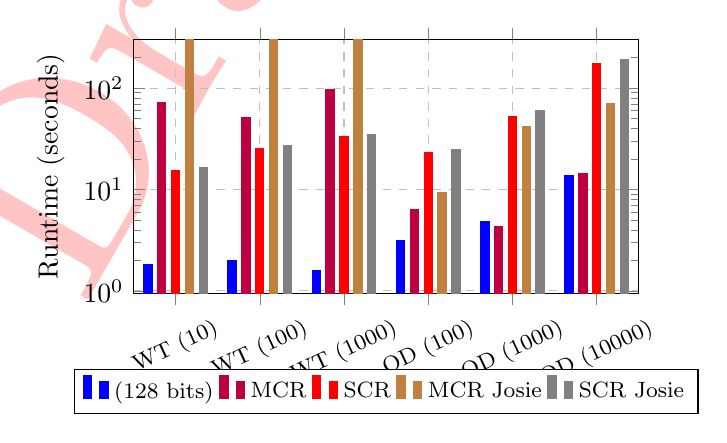
\begin{tikzpicture}
  \begin{groupplot}[xtick=data, ybar, enlarge x limits=0.1, symbolic x coords={WT (10), WT (100), WT (1000), OD (100), OD (1000), OD (10000)}, ymin = 0, group style={group size=1 by 1 , horizontal sep=.0cm}, height=4.8cm, width=8cm, ymax = 300, every node near coord/.append style={yshift=-0.21cm}, point meta=explicit symbolic, log origin=infty, xticklabel style={font=\footnotesize, rotate=25}, xmajorgrids=true, ymode = log, ytick={1, 10, 100, 1000, 10000},
    	ymajorgrids=true,grid style=dashed ]
    \nextgroupplot [ylabel={Runtime (seconds)}, 
    % legend style={legend columns=-1, at={(.95, 1)}}
    legend style={legend columns=5,at={(0.5,-0.3)},anchor=north,font=\footnotesize}
    , bar width=3pt]
    
    % \addplot[blue,fill] coordinates {(Webtable (10), 2.2) (Webtable (100), 5.4) (Webtable (1000), 4.9) (opendata (100), 2.2) (opendata (1000), 5.7) (opendata (10000), 32.5)};\addlegendentry{\hash (512 bits)};
    
    % \addplot[brown,fill] coordinates {(Webtable (10), 0) (Webtable (100), 0) (Webtable (1000), 0) (opendata (100), 4.9) (opendata (1000), 42.0) (opendata (10000), 64)}; \addlegendentry{Josie};
    
    % \addplot[red,fill] coordinates {(Webtable (10), 44.4) (Webtable (100), 55.2) (Webtable (1000), 59.9) (opendata (100), 29.8) (opendata (1000), 84.9) (opendata (10000), 503.1)}; \addlegendentry{SCI};
    
    
    % \addplot[blue,fill] coordinates {(Webtable (10), 1.0) (Webtable (100), 2.1) (Webtable (1000), 1.6) (opendata (100), .7) (opendata (1000), 2.7) (opendata (10000), 13)};\addlegendentry{\hash (512 bits)};
    
    % \addplot[brown,fill] coordinates {(Webtable (10), 0) (Webtable (100), 0) (Webtable (1000), 0) (opendata (100), 4.9) (opendata (1000), 42.0) (opendata (10000), 64)}; \addlegendentry{Multi-column Josie};
    
    % \addplot[red,fill] coordinates {(Webtable (10), 15.5) (Webtable (100), 25.4) (Webtable (1000), 33.5) (opendata (100), 22.9) (opendata (1000), 52.0  ) (opendata (10000), 175.6)}; \addlegendentry{SCI+Filtering};
    
    % \addplot[gray,fill] coordinates {(Webtable (10), 0) (Webtable (100), 0) (Webtable (1000), 0) (opendata (100), 26.16) (opendata (1000), 62.37) (opendata (10000), 196.08)}; \addlegendentry{Josie+Filtering};
    
    % \addplot[purple,fill] coordinates {(Webtable (10), 100.6) (Webtable (100), 82.70) (Webtable (1000), 140.8) (opendata (100), 12.8) (opendata (1000), 7.1) (opendata (10000), 19.60)}; \addlegendentry{Multi-column SCI};
    
    \addplot[blue,fill] coordinates {(WT (10), 1.8) (WT (100), 2.0) (WT (1000), 1.6) (OD (100),3.1) (OD (1000), 4.8) (OD (10000), 13.6)};\addlegendentry{\hash (128 bits)};
    
     \addplot[purple,fill] coordinates {(WT (10), 72.4) (WT (100), 51) (WT (1000), 97.6) (OD (100), 6.3) (OD (1000), 4.3) (OD (10000), 14.40)}; \addlegendentry{MCR};
    
    \addplot[red,fill] coordinates {(WT (10), 15.5) (WT (100), 25.4) (WT (1000), 33.5) (OD (100), 22.9) (OD (1000), 52.0) (OD (10000), 175.6)}; \addlegendentry{SCR};
    
    \addplot[brown,fill] coordinates {(WT (10), 300) (WT (100), 300) (WT (1000), 300)(OD (100), 9.4) (OD (1000), 42.0) (OD (10000), 71)}; \addlegendentry{MCR Josie};
    
    \addplot[gray,fill] coordinates {(WT (10), 16.6) (WT (100), 27.3) (WT (1000), 35) (OD (100), 24.7) (OD (1000), 60) (OD (10000), 191.8)}; \addlegendentry{SCR Josie};
    
  \end{groupplot}
\end{tikzpicture}
% \vspace{-.4cm}
\caption{Runtime comparison between \system and SCI.}
\label{fig:dxf_vs_mate_runtime}
%\vspace{-.2cm}
\end{figure}


%Here, we only report the runtime for the 512-bit version of \system.
%Later in this section, we also evaluate the system performance for hash arrays with varied sizes.
Figure~\ref{fig:dxf_vs_mate_runtime} shows the runtime comparison \system against SCR, MCR, and the corresponding JOSIE implementations in log scale.
Without the row filtering optimization of \system, the runtime for joinability calculation dominates the overall runtime.
The depicted runtime results for baselines include the time required to discover the multi-column joins in-memory on top of the state-of-the-art single-attribute joinable table discovery systems. 
Note that there is an additional fetching cost that is negligible, i.e.,~in the order of milliseconds when we use the in-memory implementation like state-of-the-art~\cite{zhu2019josie}. However, the fetching cost can vary between $1$ and $40$ seconds when the data and the index has to be retrieved from disk. This is the case for the DWTC, which cannot fit into memory. The depicted runtime does not contain the fetching time as it is the same for both approaches.
We observe that \system outperforms baseline systems in almost all experiments: it is up to $61x$, $13x$, $9x$, $22x$ faster than MCR, SCR, MCR Josie, and SCR Josie respectively.
%As a result, it can drop most of the non-joinable table rows before any further computation.
This experiment also shows that no other baseline constantly performs better than the other approaches. For instance, SCR-based approaches are slower than their corresponding MCR-based systems for open data queries but on the large webtable corpus they underperform. Note that MCR Josie for webtables did not terminate in $7$ days. The slower performance of the MCR approaches on webtable queries is because accessing the relevant PLs does not scale for the size of the webtable corpus. While MCR Josie performs similar to MCR in OD (100) its performance drops as the cardinality of the open data queries grows.
The size of the input dataset correlates with the runtime. This is expected because join columns with higher cardinality initially match more PL items in the index which again need to be fetched and filtered. 

In addition to the input table size, FPs play an important role in the number of comparisons and ultimately the runtime.
For instance, in case of SCR, although OD (1k) and WT (1k) have similar query table sizes, the OD (1k) queries lead to $35\%$ higher runtime than WT (1k). This increase in runtime is because of the large number of FPs for OD (1k) tables, i.e., $3M$ more FP rows compared to WT (1k).
%Moreover, For some query datasets, such as OD (10,000), the performance difference between \system and baselines is smaller, because the initial column filters already many of the FPs.
%On the other hand, for some datasets, such as WT (10), this performance gap is substantial because SCR retrieves over one orders of magnitude more FPs than \system. % 400 times more
\newline
\textbf{Summary.}
(i) \system is up to $100x$ faster than unary join discovery systems in discovering n-ary joins.
(ii) Performance gain of \system over SCR-based approaches depends on the number of FP rows.


\subsection{\hash VS. Baseline Hash Functions} \label{subsubsec:xash_vs_hashes}
Table~\ref{tab:dataset_runtime} depicts the runtime of \system with different hash functions, including the proposed \hash.
Note that all the competing hash functions benefit from all of \system's optimizations and only differ in the applied hash function during row filtering.

% \begin{table*}[]
%      \footnotesize
%     \centering
%     \caption{Runtime experiment (seconds). \colorbox[HTML]{A2EDFF}{blue} cells represent the experiments where the larger hash performs worse. \colorbox[HTML]{FFABA8}{Red} cells show the maximum performance gain of \system over BF.}
%     \label{tab:dataset_runtime}
% \begin{tabular}{r|r|r|r|r|rrr|rrr|rrr|rrr|rrr}
% \toprule
% \textit{\textbf{Dataset}} &
% \textit{\textbf{SCR}}&\textit{\textbf{\thead{MD5}}}&\textit{\textbf{{Murmur}}}&\textit{\textbf{{CityHash}}}&
%  \multicolumn{3}{c|}{\textit{\textbf{{SimHash}}}}& \multicolumn{3}{c|}{\textit{\textbf{{HT}}}}& \multicolumn{3}{c|}{\textit{\textbf{{BF}}}}& \multicolumn{3}{c|}{\textit{\textbf{{LHBF}}}}&  \multicolumn{3}{c}{\textit{\textbf{{\hash}}}}
%  \\

% &&\multicolumn{1}{c|}{\textbf{128}}&\multicolumn{1}{c|}{\textbf{128}}&\multicolumn{1}{c|}{\textbf{128}}&\multicolumn{1}{c}{\textbf{128}}&\multicolumn{1}{c}{\textbf{256}}&\multicolumn{1}{c|}{\textbf{512}}&\multicolumn{1}{c}{\textbf{128}}&\multicolumn{1}{c}{\textbf{256}}&\multicolumn{1}{c|}{\textbf{512}}&\multicolumn{1}{c}{\textbf{128}}&\multicolumn{1}{c}{\textbf{256}}&\multicolumn{1}{c|}{\textbf{512}}&\multicolumn{1}{c}{\textbf{128}}&\multicolumn{1}{c}{\textbf{256}}&\multicolumn{1}{c|}{\textbf{512}}&\multicolumn{1}{c}{\textbf{128}}&\multicolumn{1}{c}{\textbf{256}}&\multicolumn{1}{c}{\textbf{512}}\\
% \toprule
% WT (10) & 15.5 & 8.6 & 8.4 & 8.6 & {7.0}&\colorbox[HTML]{A2EDFF}{8.0}& 4.1 & {4.3}&\colorbox[HTML]{A2EDFF}{6.3}& 3.1 & {2.5}&\colorbox[HTML]{A2EDFF}{3.0}& 1.6  & {2.9}&\colorbox[HTML]{A2EDFF}{3.2}& 2.1  & \textbf{1.0}&\textbf{1.0}&\textbf{0.7}  \\

% WT (100) & 25.4 & 15.7 & 15.2 & 15.7 & 13.7&8.5&6.1 & {9.6}&\colorbox[HTML]{A2EDFF}{10.2}&4.1 & {4.9}&\colorbox[HTML]{A2EDFF}{5.3}&2.8 &{5.7} &{3.5}&\colorbox[HTML]{A2EDFF}{4.4}& {\textbf{1.6}}&\colorbox[HTML]{A2EDFF}{\textbf{1.8}}&\textbf{1.2}\\

% WT (1000) & 33.5 & 20.8 & 20.5 & 20.4 & 17.2&10.2&6.9 & {13.7}& \colorbox[HTML]{A2EDFF}{13.9}&5.3 & 5.7&5.5&{2.4} & 7.5&{4.1}&\colorbox[HTML]{A2EDFF}{4.6} & \textbf{1.6}&\textbf{1.5}&{\textbf{1.2}} \\

% \toprule

% OD (100) & 22.9 & {22.0} & 21.7 & 21.9 & {20.8}&\colorbox[HTML]{A2EDFF}{22.8}&{21.1} & 7.8&6.7&4.5 & 4.2&2.6&\colorbox[HTML]{FFABA8}{1.8} & 6.2 &4.8&2.9& \textbf{3.5}&\textbf{1.0}&\colorbox[HTML]{FFABA8}{\textbf{0.7}}\\

% OD (1000) & 52.0 & 50.4 & 49.8 & 51.1 & {47.9}&\colorbox[HTML]{A2EDFF}{49.4}&43.95 & 17.1&16.5&13.2 & 10.9&6.5&4.8 & 15.5&12.0&8.3 & \textbf{7.0}&\textbf{3.1}&\textbf{2.7} \\

% OD (10000) & 175.6 & {137.4} & {130.2} & {131.9} & {123.9}&120.2&99.4 & 44.6&44.6&33.5 & 28.2&18.8&15.1 & 36.3&29.3&22.2 & \textbf{18}&\textbf{13.3}&\textbf{13}\\
% \toprule
% Kaggle & 297.0 & 97.6 &104.2&104.4&{76.6}&57.3&41.0&34.8&30.3&25.9&19.7&14.8&13.1 & 37.8&27.1&21.8&\textbf{15.2}&\textbf{12.0}&{\textbf{12.3}}\\
% \toprule
% School & 873.6 & 772.7 & 772.9 & 742.8 & 593.7&444.0&307.2 & 54.3&38.3&31.0 & 24.2&19.0& 19.0 & 33.8&25.3&22.7 &\textbf{20.0}&\textbf{17.9}&\textbf{17.6}\\
% \end{tabular}
% \end{table*}



\begin{table*}[]
     \footnotesize
    \centering
    \caption{Runtime experiment (seconds). \colorbox[HTML]{A2EDFF}{blue} cells represent the experiments where the larger hash performs worse. \colorbox[HTML]{FFABA8}{Red} cells show the maximum performance gain of \system over BF.}
    % \vspace{-.2cm}
    \label{tab:dataset_runtime}
\begin{tabular}{r|r|r|r|r|rrr|rrr|rrr|rrr|rrr}
%\toprule
\textit{\textbf{Dataset}} &
\textit{\textbf{SCR}}&\textit{\textbf{\thead{MD5}}}&\textit{\textbf{{Murmur}}}&\textit{\textbf{{City}}}&
 \multicolumn{3}{c|}{\textit{\textbf{{SimHash}}}}& \multicolumn{3}{c|}{\textit{\textbf{{HT}}}}& \multicolumn{3}{c|}{\textit{\textbf{{BF}}}}& \multicolumn{3}{c|}{\textit{\textbf{{LHBF}}}}&  \multicolumn{3}{c}{\textit{\textbf{{\hash}}}}
 \\

&&\multicolumn{1}{c|}{\textbf{128}}&\multicolumn{1}{c|}{\textbf{128}}&\multicolumn{1}{c|}{\textbf{128}}&\multicolumn{1}{c}{\textbf{128}}&\multicolumn{1}{c}{\textbf{256}}&\multicolumn{1}{c|}{\textbf{512}}&\multicolumn{1}{c}{\textbf{128}}&\multicolumn{1}{c}{\textbf{256}}&\multicolumn{1}{c|}{\textbf{512}}&\multicolumn{1}{c}{\textbf{128}}&\multicolumn{1}{c}{\textbf{256}}&\multicolumn{1}{c|}{\textbf{512}}&\multicolumn{1}{c}{\textbf{128}}&\multicolumn{1}{c}{\textbf{256}}&\multicolumn{1}{c|}{\textbf{512}}&\multicolumn{1}{c}{\textbf{128}}&\multicolumn{1}{c}{\textbf{256}}&\multicolumn{1}{c}{\textbf{512}}\\
\toprule
WT (10) & 20.6 & 12.5 & 12.6 & 12.6 & 11.1 & 10.1 & \colorbox[HTML]{A2EDFF}{12.5} & 6.4 & \colorbox[HTML]{A2EDFF}{7.3} & \colorbox[HTML]{A2EDFF}{7.6} & 4.2 & 4.2 & \colorbox[HTML]{A2EDFF}{10.3} & 4.1 & 3.6 & 2.2 & \textbf{1.8} & \textbf{1.5} & \textbf{1.4} \\
WT (100) & 24.5 & 15.3 & 14.8 & 15.3 & 13.4 & 8.5 & \colorbox[HTML]{A2EDFF}{17.2} & 9.5 & \colorbox[HTML]{A2EDFF}{10.1} & \colorbox[HTML]{A2EDFF}{12.4} & 4.7 & \colorbox[HTML]{A2EDFF}{5.0} & \colorbox[HTML]{A2EDFF}{16.8} & 5.6 & 3.6 & \colorbox[HTML]{A2EDFF}{4.2} & \textbf{1.6} & \colorbox[HTML]{A2EDFF}{\textbf{1.8}} & \colorbox[HTML]{A2EDFF}{\textbf{2.0}}\\
WT (1k) & 32.7 & 20.2 & 19.8 & 19.8 & 16.3 & 10.0 & \colorbox[HTML]{A2EDFF}{17.0} & 13.4 & \colorbox[HTML]{A2EDFF}{13.8} & 13.4 & 5.6 & 5.5 & \colorbox[HTML]{FFABA8}{16.7} & 7.6 & 4.1 & \colorbox[HTML]{A2EDFF}{4.6} & \textbf{1.6} & \textbf{1.5} & \colorbox[HTML]{FFABA8}{\textbf{1.6}}\\
\toprule
OD (100) & 247.6 & 212.1 & 224.2 & 194.5 & 102.9 & 69.1 & 56.5 & 24.0 & 16.4 & 10.8 & 11.0 & 4.8 & 3.4 & 30.1 & 9.5 & 8.3 & \textbf{6.5} & \textbf{3.5} & \textbf{3.}1\\
OD (1k) & 165.8 & 146.8 & 152.3 & 138.6 & 90.0 & 73.6 & 62.6 & 25.4 & 21.6 & 16.5 & 14.4 & 7.6 & 5.6 & 39.2 & 11.3 & \colorbox[HTML]{A2EDFF}{13.0} & \textbf{8.7} & \textbf{4.5} & \colorbox[HTML]{A2EDFF}{\textbf{4.8}}\\
OD (10k) & 256.7 & 203.9 & 202.1 & 190.6 & 145.6 & 127.0 & 103.5 & 49.6 & 44.0 & 31.9 & 27.7 & 17.8 & 14.3 & 79.2 & 27.0 & 21.8 & \textbf{17.6} & \textbf{13.4} & \colorbox[HTML]{A2EDFF}{\textbf{13.6}}\\
\toprule
Kaggle & 297.0 & 97.6 &104.2&104.4&{76.6}&57.3&41.0&34.8&30.3&25.9&19.7&14.8&13.1 & 37.8&27.1&21.8&\textbf{15.2}&\textbf{12.0}&{\textbf{12.3}}\\
\toprule
School & 873.6 & 772.7 & 772.9 & 742.8 & 593.7&444.0&307.2 & 54.3&38.3&31.0 & 24.2&19.0& 19.0 & 33.8&25.3&22.7 &\textbf{20.0}&\textbf{17.9}&\textbf{17.6}\\
\end{tabular}
\end{table*}
% \begin{table*}[]
%     % \vspace{-.2cm}
%     \footnotesize
%     \centering
%     \caption{Precision experiment.}
%         \vspace{-.1cm}
%     \label{tab:dataset_precision}
% \begin{tabular}{r|rrrrrrr|rrrrr}
% \toprule
% \textit{\textbf{Dataset}} & \textit{\textbf{\thead{MD5\\Murmur\\(128)}}}&\textit{\textbf{\thead{CityHash \\ (128)}}} & \textit{\textbf{\thead{SimHash \\(128)}}}& \textit{\textbf{\thead{HT \\ (128)}}}& \textit{\textbf{\thead{BF \\(128)}}}&\textit{\textbf{\thead{LHBF \\(128)}}}& \textit{\textbf{\thead{\hash \\ (128)}}}&
% \textit{\textbf{\thead{SimHash \\(512)}}}&\textit{\textbf{\thead{HT \\ (512)}}}& \textit{\textbf{\thead{BF \\(512)}}}&\textit{\textbf{\thead{LHBF \\(512)}}}& \textit{\textbf{\thead{\hash \\ (512)}}}\\ \toprule

% WT (10) & 0.28$\pm$0.40 & 0.28$\pm$0.40 & 0.30$\pm$0.41 & 0.34$\pm$0.43 & 0.45$\pm$0.46 & 0.44$\pm$0.44 & \textbf{0.58$\pm$0.46} & 0.35$\pm$0.43 & 0.43$\pm$0.46 & 0.62$\pm$0.45 &  0.61$\pm$0.46 & \textbf{0.94$\pm$0.20}\\
% WT (100) & 0.26$\pm$0.40 & 0.27$\pm$0.40 & 0.27$\pm$0.40 & 0.34$\pm$0.41 & 0.45$\pm$0.44 &  0.45$\pm$0.43 & \textbf{0.60$\pm$0.44} & 0.33$\pm$0.42 & 0.45$\pm$0.43 & 0.69$\pm$0.42  &  0.60$\pm$0.45 & \textbf{0.95$\pm$0.20}\\
% WT (1000) & 0.22$\pm$0.35 & 0.22$\pm$0.35 & 0.24$\pm$0.35 & 0.37$\pm$0.37 & 0.56$\pm$0.40 &  0.51$\pm$0.39 & \textbf{0.76$\pm$0.35} & 0.34$\pm$0.39 & 0.53$\pm$0.39 & 0.79$\pm$0.35 &  0.75$\pm$0.37 & \textbf{0.98$\pm$0.10}\\
% \toprule
% OD (100) & 0.36$\pm$0.42 & 0.36$\pm$0.42 & 0.37$\pm$0.42 & 0.54$\pm$0.40 & 0.66$\pm$0.41 &  0.62$\pm$0.41 & \textbf{0.77$\pm$0.38} & 0.39$\pm$0.41 & 0.67$\pm$0.40 & 0.86$\pm$0.30 &  0.78$\pm$0.35 & \textbf{0.97$\pm$0.13}\\
% OD (1000) & 0.37$\pm$0.43 & 0.37$\pm$0.43 & 0.37$\pm$0.42 & 0.53$\pm$0.41 & 0.65$\pm$0.40 &  0.63$\pm$0.42 & \textbf{0.75$\pm$0.37} & 0.46$\pm$0.42 & 0.68$\pm$0.41 & 0.90$\pm$0.26 &  0.76$\pm$0.36 & \textbf{0.97$\pm$0.15}\\
% OD (10000) & 0.37$\pm$0.43 & 0.37$\pm$0.43 & 0.37$\pm$0.42 & 0.53$\pm$0.41 & 0.65$\pm$0.40 &  0.50$\pm$0.40 & \textbf{0.75$\pm$0.37} & 0.46$\pm$0.42 & 0.66$\pm$0.41 & 0.90$\pm$0.26 &  0.72$\pm$0.36 & \textbf{0.97$\pm$0.15}\\
% \toprule
% Kaggle & 0.09$\pm$0.18&   0.09$\pm$0.17&   0.12$\pm$0.21&  0.25$\pm$0.31&  0.40$\pm$0.41&  0.33$\pm$0.34 &  \textbf{0.64$\pm$0.34}&   0.20$\pm$0.31&    0.44$\pm$0.37&    0.64$\pm$0.38 & 0.63$\pm$0.36 & \textbf{0.93$\pm$0.10}\\
% \toprule
% School & 0.00$\pm$0.00&   0.00$\pm$0.00&   0.00$\pm$0.00&  0.01$\pm$0.01&  0.07$\pm$0.03&  0.02$\pm$0.01 &  \textbf{0.43$\pm$0.11}&   0.00$\pm$0.00&    0.03$\pm$0.02&    \textbf{1.00$\pm$0.00} & 0.24$\pm$0.08 & 0.96$\pm$0.02\\
% \toprule
% Average &    0.24$\pm$0.33&   0.25$\pm$0.33&   0.26$\pm$0.33&  0.36$\pm$0.34&  0.49$\pm$0.37&  0.44$\pm$0.36 &  \textbf{0.66$\pm$0.35}&       0.32$\pm$0.35&    0.49$\pm$0.36&    0.80$\pm$0.30 & 0.64$\pm$0.35 & \textbf{0.96$\pm$0.13} \\

% \end{tabular}
% \end{table*}



% \begin{table*}[]
%     % \vspace{-.2cm}
%     \footnotesize
%     \centering
%     \caption{Precision experiment.}
%         \vspace{-.1cm}
%     \label{tab:dataset_precision}
% \begin{tabular}{r|rrrrrrr|rrrrr}
% \toprule
% \textit{\textbf{Dataset}} & \textit{\textbf{\thead{MD5\\Murmur\\(128)}}}&\textit{\textbf{\thead{CityHash \\ (128)}}} & \textit{\textbf{\thead{SimHash \\(128)}}}& \textit{\textbf{\thead{HT \\ (128)}}}& \textit{\textbf{\thead{BF \\(128)}}}&\textit{\textbf{\thead{LHBF \\(128)}}}& \textit{\textbf{\thead{\hash \\ (128)}}}&
% \textit{\textbf{\thead{SimHash \\(512)}}}&\textit{\textbf{\thead{HT \\ (512)}}}& \textit{\textbf{\thead{BF \\(512)}}}&\textit{\textbf{\thead{LHBF \\(512)}}}& \textit{\textbf{\thead{\hash \\ (512)}}}\\ \toprule

% WT (10) & 0.27$\pm$0.39 & 0.25$\pm$0.38 & 0.28$\pm$0.40 & 0.34$\pm$0.43 & 0.44$\pm$0.46 & 0.44$\pm$0.45 & \textbf{0.57$\pm$0.46} & 0.31$\pm$0.42 & 0.28$\pm$0.43 & 0.40$\pm$0.43 & 0.61$\pm$0.46 & \textbf{0.88$\pm$0.26}   \\
% WT (100) & 0.27$\pm$0.40 & 0.27$\pm$0.40 & 0.27$\pm$0.40 & 0.34$\pm$0.41 & 0.46$\pm$0.44 & 0.45$\pm$0.43 & \textbf{0.61$\pm$0.43} & 0.27$\pm$0.39 & 0.38$\pm$0.41 & 0.34$\pm$0.41 & 0.63$\pm$0.44 & \textbf{0.93$\pm$0.22}   \\
% WT (1000) & 0.24$\pm$0.36 & 0.24$\pm$0.36 & 0.25$\pm$0.37 &  0.40$\pm$0.37 & 0.59$\pm$0.39 & 0.52$\pm$0.38 & \textbf{0.77$\pm$0.34} &  0.28$\pm$0.35 & 0.42$\pm$0.36 & 0.32$\pm$0.35 & 0.78$\pm$0.33 & \textbf{0.98$\pm$0.10} \\
% \toprule
% OD (100) & 0.27$\pm$0.38 & 0.28$\pm$0.39 & 0.28$\pm$0.38 & 0.43$\pm$0.40 & \textbf{0.56$\pm$0.41} & 0.45$\pm$0.43 & 0.52$\pm$0.41 & 0.32$\pm$0.41 & 0.55$\pm$0.41 & 0.79$\pm$0.34 & 0.67$\pm$0.35 & \textbf{0.80$\pm$0.34}   \\
% OD (1000) & 0.32$\pm$0.40 & 0.32$\pm$0.40 & 0.32$\pm$0.39 & 0.47$\pm$0.40 & \textbf{0.61$\pm$0.40} & 0.44$\pm$0.34 & 0.53$\pm$0.41 & 0.41$\pm$0.41 & 0.59$\pm$0.41 & 0.85$\pm$0.28 & 0.63$\pm$0.39 & \textbf{0.86$\pm$0.28}   \\
% OD (10000) & 0.27$\pm$0.38 & 0.28$\pm$0.38 & 0.28$\pm$0.37 & 0.42$\pm$0.39 & \textbf{0.59$\pm$0.40} & 0.40$\pm$0.42 & 0.52$\pm$0.42 & 0.34$\pm$0.39 & 0.56$\pm$0.39 & \textbf{0.87$\pm$0.27} & 0.66$\pm$0.40 & 0.82$\pm$0.32   \\
% \toprule
% School & 0.00$\pm$0.00&   0.00$\pm$0.00&   0.00$\pm$0.00&  0.01$\pm$0.01&  0.07$\pm$0.03&  0.02$\pm$0.01 &  \textbf{0.43$\pm$0.11}&   0.00$\pm$0.00&    0.03$\pm$0.02&    \textbf{1.00$\pm$0.00} & 0.24$\pm$0.08 & 0.96$\pm$0.02\\
% \toprule
% Kaggle & 0.09$\pm$0.18&   0.09$\pm$0.17&   0.12$\pm$0.21&  0.25$\pm$0.31&  0.40$\pm$0.41&  0.33$\pm$0.34 &  \textbf{0.64$\pm$0.34}&   0.20$\pm$0.31&    0.44$\pm$0.37&    0.64$\pm$0.38 & 0.63$\pm$0.36 & \textbf{0.93$\pm$0.10}\\
% \toprule
% Average &    0.24$\pm$0.33&   0.25$\pm$0.33&   0.26$\pm$0.33&  0.36$\pm$0.34&  0.49$\pm$0.37&  0.44$\pm$0.36 &  \textbf{0.66$\pm$0.35}&       0.32$\pm$0.35&    0.49$\pm$0.36&    0.80$\pm$0.30 & 0.64$\pm$0.35 & \textbf{0.96$\pm$0.13} \\

% \end{tabular}
% \end{table*}






\begin{table*}[]
     \footnotesize
    \centering
    \caption{Precision experiment.}
    % \vspace{-.2cm}
    \label{tab:dataset_precision}
\begin{tabular}{r|c|c|rr|rr|rr|rr|rr}
%\toprule
\textit{\textbf{Dataset}} &
\textit{\textbf{\thead{MD5}}}&\textit{\textbf{{CityHash}}}&
 \multicolumn{2}{c|}{\textit{\textbf{{SimHash}}}}& \multicolumn{2}{c|}{\textit{\textbf{{HT}}}}& \multicolumn{2}{c|}{\textit{\textbf{{BF}}}}& \multicolumn{2}{c|}{\textit{\textbf{{LHBF}}}}&  \multicolumn{2}{c}{\textit{\textbf{{\hash}}}}
 \\

&\multicolumn{1}{c|}{\textbf{128}}&\multicolumn{1}{c|}{\textbf{128}}&\multicolumn{1}{c}{\textbf{128}}&\multicolumn{1}{c|}{\textbf{512}}&\multicolumn{1}{c}{\textbf{128}}&\multicolumn{1}{c|}{\textbf{512}}&\multicolumn{1}{c}{\textbf{128}}&\multicolumn{1}{c|}{\textbf{512}}&\multicolumn{1}{c}{\textbf{128}}&\multicolumn{1}{c|}{\textbf{512}}&\multicolumn{1}{c}{\textbf{128}}&\multicolumn{1}{c}{\textbf{512}}\\
\toprule
WT (10) & 0.27$\pm$0.39 & 0.25$\pm$0.38 & 0.28$\pm$0.40 &0.31$\pm$0.42& 0.34$\pm$0.43 &0.28$\pm$0.43 & 0.44$\pm$0.46 &0.40$\pm$0.43 & 0.44$\pm$0.45 & 0.61$\pm$0.46& \textbf{0.57$\pm$0.46} & \textbf{0.88$\pm$0.26}   \\
WT (100) & 0.27$\pm$0.40 & 0.27$\pm$0.40 & 0.27$\pm$0.40 &0.27$\pm$0.39 & 0.34$\pm$0.41 &0.38$\pm$0.41 & 0.46$\pm$0.44 &0.34$\pm$0.41  & 0.45$\pm$0.43 & 0.63$\pm$0.44& \textbf{0.61$\pm$0.43} &\textbf{0.93$\pm$0.22} \\
WT (1k) & 0.24$\pm$0.36 & 0.24$\pm$0.36 & 0.25$\pm$0.37 & 0.28$\pm$0.35 &  0.40$\pm$0.37 &0.42$\pm$0.36 &  0.59$\pm$0.39 & 0.32$\pm$0.35&  0.52$\pm$0.38  &0.78$\pm$0.33 & \textbf{0.77$\pm$0.34} &\textbf{0.98$\pm$0.10}  \\
\toprule
OD (100) & 0.27$\pm$0.38 & 0.28$\pm$0.39 & 0.28$\pm$0.38 &0.32$\pm$0.41 & 0.43$\pm$0.40 &0.55$\pm$0.41 & \textbf{0.56$\pm$0.41} & 0.79$\pm$0.34& 0.45$\pm$0.43 &0.67$\pm$0.35 & 0.52$\pm$0.41 & \textbf{0.80$\pm$0.34}   \\
OD (1k) & 0.32$\pm$0.40 & 0.32$\pm$0.40 & 0.32$\pm$0.39 &0.41$\pm$0.41 & 0.47$\pm$0.40 &0.59$\pm$0.41 & \textbf{0.61$\pm$0.40} &0.85$\pm$0.28 & 0.44$\pm$0.34 & 0.63$\pm$0.39 & 0.53$\pm$0.41 & \textbf{0.86$\pm$0.28}   \\
OD (10k) & 0.27$\pm$0.38 & 0.28$\pm$0.38 & 0.28$\pm$0.37 & 0.34$\pm$0.39& 0.42$\pm$0.39 &0.56$\pm$0.39 & \textbf{0.59$\pm$0.40} & \textbf{0.87$\pm$0.27}& 0.40$\pm$0.42 & 0.66$\pm$0.40& 0.52$\pm$0.42 & 0.82$\pm$0.32   \\
\toprule
School & 0.00$\pm$0.00&   0.00$\pm$0.00&   0.00$\pm$0.00 & 0.00$\pm$0.00 & 0.01$\pm$0.01& 0.03$\pm$0.02 & 0.07$\pm$0.03&  \textbf{1.00$\pm$0.00} & 0.02$\pm$0.01 & 0.24$\pm$0.08 & \textbf{0.43$\pm$0.11}& 0.96$\pm$0.02\\
\toprule
Kaggle & 0.09$\pm$0.18&   0.09$\pm$0.17&   0.12$\pm$0.21 &  0.20$\pm$0.31 &  0.25$\pm$0.31& 0.44$\pm$0.37 &  0.40$\pm$0.41&  0.64$\pm$0.38 &  0.33$\pm$0.34 & 0.63$\pm$0.36 &  \textbf{0.64$\pm$0.34}& \textbf{0.93$\pm$0.10}\\
\toprule
Average &    0.22$\pm$0.31&   0.22$\pm$0.31&   0.23$\pm$0.32&  0.27$\pm$0.34&  0.33$\pm$0.34&  0.41$\pm$0.35 &  0.47$\pm$0.37&       0.65$\pm$0.31&    0.38$\pm$0.35&    0.61$\pm$0.35 & \textbf{0.57$\pm$0.37} & \textbf{0.90$\pm$0.21} \\
\end{tabular}
\end{table*}
In Table~\ref{tab:dataset_runtime}, we highlight the best performing approach of each row and hash size in \textbf{bold} font.
We observe that \system with \hash outperforms all the other baselines on all of the queries.
%\hash leverages simple syntactic information of the cell values to generate distinguishable index elements. 
\system + \hash can be up to $10x$ faster than \system + BF, which is the second most efficient baseline on average.
The cells showing this speedup are highlighted with \colorbox[HTML]{FFABA8}{red}.
BF's under-performance is rooted in its higher collision rate compared to \hash. Besides, by checking the length attribute that we use in \hash to generate the hash results, we can drop many of the non-joinable rows without evaluating all the bits in the super keys. This feature gives \system a superiority over BF in runtime even in the cases with similar or lower FP rates.
Another interesting insight is that \system + BF is faster than \system + HT in most of the cases and this is because BF is able to leverage more bits in the hash space to encode the join keys than a hash table that leverages only a single bit to hash each key value.%A single bit can only generate a limited number of unique hash values, e.g., 128 different hash values in 128-bit hash space, therefore, in the best case, $\frac{1}{128}$ of the single hashes will lead to collision, i.e., the same hash value. 
Table~\ref{tab:dataset_runtime} shows that \hash performs also better than LHBF in all of the cases. LHBF leverages fewer hash functions in comparison to BF with statistically similar FP probability. However, similar to HT, fewer hashing does not necessarily lead to a better performance in discovering the joinable tables. In our experiments LHBF only performs better on larger hash sizes for webtable queries, but in the remaining cases, LHBF is less efficient than BF.

The results also show that although super keys based on the standard hash functions, MD5, CityHash, SimHash, and Murmur, lead to overall performance gains over the naive SCR approach, all of them clearly fall behind \hash.
This is because they are not optimized to identify subset relationships that we encode via bitwise OR masking. They generate too many 1 bits (on average $50\%$) in the hash results, which leads to a higher number of FPs.
Thus, if a table contains six columns the aggregation of six hash results will on average turn $98\%$ of the super key to 1s, which would make the super key highly ineffective in masking.

%MD5, CityHash, SimHash, and Murmur lead to a very similar performance to SCR specially in open data and school experiments. This performance drop is because the row filtering overhead is almost as high as the runtime benefit from the row filtering.

Further, the experiments show that in most of the cases, a larger hash size (512 bits) leads to a faster join discovery than the smaller versions. However, in cases such as WT (100) and Simhash, the larger hash size results in slower discovery. The experiments that lead to slower runtime compared to their smaller hash size are marked as \colorbox[HTML]{A2EDFF}{blue} cells. 
When the FP rate is similar for two hash sizes, the approach with the larger hash size will result in similar or higher runtime. 
This is because the bit-wise OR operation is more expensive for larger hash values.
For instance, for WT (100) query tables and SimHash, the difference between the FP rate is almost zero, therefore, the runtime overhead of 512-bit hash causes worse performance.
In the more common case that a larger hash size reduces the number of FPs the resulting runtime is also lower.
For example, for the OD (100) datasets, the larger hash size for \hash results in $85\%$ fewer FPs on average, leading to $48\%$ speed-up.

Finally, we also observed that \system can indeed find interesting joinable tables based on composite keys. 
%Similarly, we observe that using composite keys we can find interesting tables for almost any dataset.  
% As another example, the most joinable table to the \textit{Page View} dataset~\cite{base_pageview} with query columns <``Name'', ``Country''>, which contains the information about Wikipedia pages of people, reveals the birth/death date of the people in the given countries. 
Searching for the top joinable tables to Kaggle Movie dataset based on a single-column join and ``Movie Title'' key columns, none of the top-10 tables contains more than one additional column, containing float numbers. However, using our multi-column join discovery approach and query columns <``Director name'', ``Movie Title''>, we obtain a table with 8 columns worth of information, including the plot of the movie, actor names, etc.
For the \textit{Kaggle Airline} dataset with join keys ``Airline name'' and ``Country'' \system obtains a table representing the airports in which the airlines operate flights in the given countries. 

\noindent\textbf{Summary.}
(i)~The syntactic feature extraction in \hash leads to a faster multi-attribute join discovery compared to the baselines;
(ii)~the standard hash functions are not ideal for n-ary joins due to their uniform distribution property that results in too many 1 bits; and
(iii)~ larger hash sizes result in higher calculation overhead.

\subsection{FP Rate}\label{subsubsection:fp}
%We now delve into more details regarding the FP rates.
There is a direct relationship between the table discovery runtime and the FP rate of the hash function used.
We measure the precision as the ratio of true positives (TP) over both TPs and FPs: $precision = \frac{TP}{TP + FP}$. Precision normalizes the TP-rate across datasets.

Table~\ref{tab:dataset_precision} shows the results of this experiment. Due to space reasons in this experiment, we only show the results for $128$- and $512$-bit hash sizes. Note that we observe the same trends as the other hash sizes.
Like runtime, precision increases with larger hash sizes in most of the cases. This is due to the fact that hash functions can scatter the values in a larger range and this leads to lower collision rate between super keys.
On average, \system + \hash achieves the highest precision compared to all the other approaches both in 128- and 512-bit hash spaces. \hash achieves up to $25\%$ higher precision than BF. 
% \hash maps the character and length features of the cell values to hash bits and rotates them based on the length. This removes the random overlap between the hashes. 
However, in five cases, BF outperforms \hash. In these experiments the difference between BF and \hash is only $4\%$.
\system's runtime superiority regardless of its precision is because of the design of \hash: the length feature of the cell value is located on the left-most segment of the array. Thus, the bit-wise OR operation can skip a table row before even getting to the character features of the cell values ensuring that this happens in the very first bit-segment of the hash. If the length of the key value has never appeared in the candidate row, \system moves to the next row.
In baseline approaches, such as BF, the 0-bits are randomly scattered. Therefore, step-wise filtering might take longer to find the contradicting bits.
% For query tables, such as WT (1k), \hash leads to distinctively high precision with 128 bits. 
%\hash achieves up to $25\%$ higher precision than BF. 
\hash displays the smallest standard deviation showing its robustness in achieving high precision.
In general, the precision achieved by LHBF is consistent with its runtime performance compared to the BF approach. LHBF achieves higher precision and ultimately, lower runtime for webtable queries with $512$-bit hash sizes but in the remaining experiments BF outperforms LHBF.
%As observed before, the SimHash function performs better than the other remaining hash functions. %CityHash performs very similarly to Murmur and MD5 except on WT (100), OD (100), and OD (10k), where CityHash gains up to $2\%$ more precision.
% As the precision experiments show, BF performs better than \hash in a single case of school query tables and $512$-bits hash size. However, due to the special hash design in \hash and the segmentation of the hash array, the evaluation process in \hash is much faster than BF. In \hash, a large portion of the FPs are pruned by only checking the length bits. This optimization prevents from checking all the remaining bits and leads to faster join discovery.

\noindent\textbf{Summary.}
(i) The precision of an approach correlates with its runtime.
(iii) The segmentation of bits in \hash leads to faster join discovery even in cases where precision rates are similar.

\subsection{\system In Depth}
\subsubsection{Top-$k$.}
% \begin{figure}[t!]
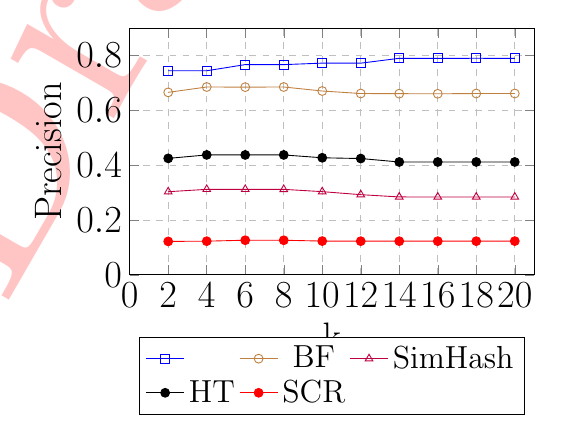
\begin{tikzpicture}[scale=0.8]
  \begin{groupplot}
    \nextgroupplot [
    	xlabel={k},
    	ylabel={Precision},
    	label style={font=\LARGE},
    	tick label style={font=\LARGE},
    	legend style={legend columns=3,at={(0.5,-0.25)},anchor=north,font=\Large},
    	width = 8cm,
    	height = 5.5cm,
    	xmin=0,
    	xmax=21,
    	ymin= 0,
    	ymax=.9,
    % 	ymode=log,
    	xtick={0, 2, 4, 6, 8, 10, 12, 14, 16, 18, 20},
    	ytick={0, .2, .4, .6, .8},
    	xmajorgrids=true,
    	ymajorgrids=true,
    	grid style=dashed]
    % 	\addplot[color=orange,mark=x] coordinates{(1,20588)(2,21069)(3,22225)(4,28451)(5,33406)(6,36650)(7,38444)(8,39346)(9,41242)(10,42847)(11,45166)(12,48807)(13,51618)(14,55643)(15,57868)(16,58111)(17,59849)(18,60661)(19,61591)(20,61883)}; \addlegendentry{True positives}
    	\addplot[color=blue,mark=square] coordinates{(2, 0.7444244234644304)(4, 0.7444460986518573)(6, 0.766964592170994)(8, 0.7668418665646705)(10, 0.7723498169274685)(12, 0.7721850123943121)(14, 0.789895797886049)(16, 0.7898665438117544)(18, 0.7899121864602451)(20, 0.7898665438117544)
}; \addlegendentry{\hash}
    	\addplot[color=brown,mark=o] coordinates{(2, 0.6657185337122508)(4, 0.6852987283763192)(6, 0.6847869632839787)(8, 0.6853100974388263)(10, 0.6706663366294509)(12, 0.6615030786875513)(14, 0.6609914966790925)(16, 0.6605009207276907)(18, 0.6615030239812544)(20, 0.6615030968085653)
}; \addlegendentry{BF}
    % 	\addplot[color=green,mark=otimes] coordinates{(1, 0.008487964801414276)(2, 0.00867506847329665)(3, 0.009056228892568881)(4, 0.011118979450347002)(5, 0.010706217432424333)(6, 0.010493747272771001)(7, 0.01087875580809653)(8, 0.010654525140330435)(9, 0.010256007269375988)(10, 0.010313630953168985)(11, 0.009810088365946748)(12, 0.009603656106980404)(13, 0.009668111695178587)(14, 0.010120234047804433)(15, 0.010479001253467317)(16, 0.010491242012774505)(17, 0.010487978665500265)(18, 0.01042295610506084)(19, 0.010553417433743212)(20, 0.010502225759753715)}; \addlegendentry{MD5}
    	\addplot[color=purple,mark=triangle] coordinates{(2, 0.30345662577661975)(4, 0.312138456555909)(6, 0.31220590396905923)(8, 0.31208672045033997)(10, 0.3036917898770219)(12, 0.2926698617018144)(14, 0.28438747405412956)(16, 0.2843694657737292)(18, 0.2843812923475462)(20, 0.28436718822604207)
}; \addlegendentry{SimHash}
        \addplot[color=black,mark=*] coordinates{(2, 0.42501046760605)(4, 0.43763678480021895)(6, 0.4375524593109754)(8, 0.43756087888715633)(10, 0.42717674533780864)(12, 0.4244305492112715)(14, 0.41187722681746775)(16, 0.411916505462486)(18, 0.4119544603091702)(20, 0.4118983532382111)
}; \addlegendentry{HT}
        \addplot[color=red,mark=*] coordinates{(2, 0.12227078467022626)(4, 0.12308378688197472)(6, 0.12659158889930547)(8, 0.12646800973130415)(10, 0.12348312509596455)(12, 0.12307493167176285)(14, 0.12310921932932725)(16, 0.12315553533822131)(18, 0.123103309723566)(20, 0.12328776753409271)
}; \addlegendentry{SCR}
		
  \end{groupplot}
\end{tikzpicture}
\caption{topk experiment.}
\label{fig:topk}
\end{figure}
The number of top-$k$ joinable tables changes the stopping criteria of the system (see table filtering step in Section~\ref{sec:index_applicaiton}).
Larger $k$ requires more tables to be evaluated.
In this experiment, we measure the precision of \system with different hash functions and vary $k$ from $2$ to $20$.
We ran the experiment with the WT (100) datasets as the input dataset against the DWTC corpus.
Other variables, such as key columns, are fixed in this experiment.
%We limit this experiment to the best performing hash functions.
In this expeirment, \system + \hash achieves the highest precision in comparison to other approaches for all $k$ values.
Increasing $k$, the precision for \hash increases $4\%$, while the precision remains the same for BF. The other hash functions lead to a slight precision cut encountering new tables with lower candidate joinable rows. This shows that \hash has higher ability to filter non-related rows compared to the given baselines. According to our observations on the candidate tables, this variation in precision occurs when the candidate tables contain more columns than average.
%Because of the reason that \hash is able to encode the cell values depending on their syntactical differences, the values from different domains map to different hash functions and these achieves fewer FPs.

% Figure~\ref{fig:topk} shows the results. \system + \hash achieves the highest precision in comparison to other approaches for all $k$ values.
% As expected, increasing $k$, increases the number of validated PL items because the first rule in the table filtering step starts later. Therefore, the system evaluates more candidate tables to discover the top-$k$ joinable tables. 
% According to the experiment, increasing $k$, the precision for \system increases, where, generally, the other hash functions lead to a slight precision cut encountering new tables with lower candidate joinable rows. This shows that \hash has higher ability to filter non-related rows compared to the given baselines. According to our observations on the candidate tables, this variation in precision occurs when the candidate tables contain more columns than average.
% Because of the reason that \hash minimizes the number of used bits in the candidate rows, the super key does not lose its ability in filtering irrelevant rows even in the existence of high dimensional tables. 
% This is not the case for BF. Because of the higher FP rate, more tables and in particular tables with large dimensions are passed to BF, which BF fails to filter.

\subsubsection{\hash components}
% \begin{figure}[t!]
% \centering
% \begin{tikzpicture}[scale=0.7]
%   \begin{groupplot}[label style={font=\LARGE},
%     	tick label style={font=\LARGE},
% % 		xlabel={Approaches},
% % 		ylabel={FP},
% % 		label style={font=\large},
% % 		tick style={font=\large},
% 		legend style={legend columns=2,at={(0.5,-0.25)},anchor=north,font=\Large},
% 	    x label style={at={(axis description cs:0.5,-0.1)},anchor=north},
% 		symbolic x coords = {Approaches},
% 		x tick label style  = {text width=1cm,align=center},
% 		xtick=data,
% 		ybar,
% % 		x=5.0cm,
%         width = 8cm,
%         height = 5cm,
% % 		bar width=5.0pt,
% 		ymin=100.0,
% 		ymode = log,
% 		ymax=400000,
% 		ytick={0.0, 10, 100, 1000, 10000, 100000, 1000000, 10000000, 10000000},
% 		xmajorgrids=true,
% 		ymajorgrids=true,
% 		grid style=dashed ]
%     \nextgroupplot [ylabel={FP}]
     
%         \addplot[fill=red] coordinates{(Approaches,103915.5)}; \addlegendentry{DXF}
% 		\addplot[fill=purple] coordinates{(Approaches,28693)}; \addlegendentry{Length}
% 		\addplot[fill=olive] coordinates{(Approaches,7563)}; \addlegendentry{Rare characters}
% 		\addplot[fill=teal] coordinates{(Approaches,2556)}; \addlegendentry{Char. + loc.}
% 		\addplot[fill=violet] coordinates{(Approaches,2435)}; \addlegendentry{Char. + len. + loc.}
% 		\addplot[fill=cyan] coordinates{(Approaches,2204)}; \addlegendentry{\hash (128 bit)}
% 		\addplot[fill=blue] coordinates{(Approaches,2047)}; \addlegendentry{\hash (512 bit)}
% 		\addplot[fill=orange] coordinates{(Approaches,2038)}; \addlegendentry{True positives}
    
%   \end{groupplot}
% \end{tikzpicture}
% %\vspace{-.2cm}
% \caption{The influence of \hash components on FP (Webtable 100).}
% \label{fig:components}
% %\vspace{-.2cm}
% \end{figure}




% # by precision
\begin{figure}[t!]
% \vspace{-.2cm}
\centering
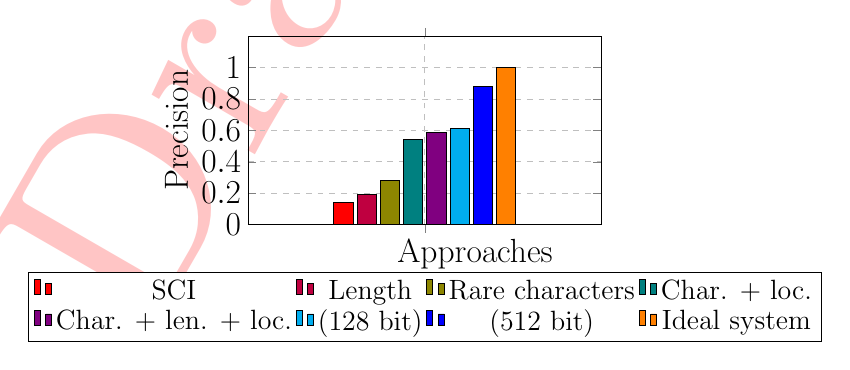
\begin{tikzpicture}[scale=0.7]
  \begin{groupplot}[label style={font=\LARGE},
    	tick label style={font=\LARGE},
% 		xlabel={Approaches},
% 		ylabel={FP},
% 		label style={font=\large},
% 		tick style={font=\large},
		legend style={legend columns=4,at={(0.5,-0.25)},anchor=north,font=\Large},
	    x label style={at={(axis description cs:0.5,-0.1)},anchor=north},
		symbolic x coords = {Approaches},
		x tick label style  = {text width=1cm,align=center},
		xtick=data,
		ybar,
% 		x=5.0cm,
        width = 8cm,
        height = 5cm,
% 		bar width=5.0pt,
		ymin=0.0,
% 		ymode = log,
		ymax=1.2,
		ytick={0.0, .2, .4, .6, .8, 1},
		xmajorgrids=true,
		ymajorgrids=true,
		grid style=dashed ]
    \nextgroupplot [ylabel={Precision}]

%         \addplot[fill=red] coordinates{(Approaches, 0.14)}; \addlegendentry{SCI}
% 		\addplot[fill=purple] coordinates{(Approaches,0.21)}; \addlegendentry{Length}
% 		\addplot[fill=olive] coordinates{(Approaches,0.31)}; \addlegendentry{Rare characters}
% 		\addplot[fill=teal] coordinates{(Approaches,0.58)}; \addlegendentry{Char. + loc.}
% 		\addplot[fill=violet] coordinates{(Approaches,0.63)}; \addlegendentry{Char. + len. + loc.}
% 		\addplot[fill=cyan] coordinates{(Approaches,0.65)}; \addlegendentry{\hash (128 bit)}
% 		\addplot[fill=blue] coordinates{(Approaches,0.89)}; \addlegendentry{\hash (512 bit)}
% 		\addplot[fill=orange] coordinates{(Approaches,1.0)}; \addlegendentry{Ideal system}


        \addplot[fill=red] coordinates{(Approaches, 0.14)}; \addlegendentry{SCI}
		\addplot[fill=purple] coordinates{(Approaches,0.19)}; \addlegendentry{Length}
		\addplot[fill=olive] coordinates{(Approaches,0.28)}; \addlegendentry{Rare characters}
		\addplot[fill=teal] coordinates{(Approaches,0.54)}; \addlegendentry{Char. + loc.}
		\addplot[fill=violet] coordinates{(Approaches,0.59)}; \addlegendentry{Char. + len. + loc.}
		\addplot[fill=cyan] coordinates{(Approaches,0.61)}; \addlegendentry{\hash (128 bit)}
		\addplot[fill=blue] coordinates{(Approaches,0.88)}; \addlegendentry{\hash (512 bit)}
		\addplot[fill=orange] coordinates{(Approaches,1.0)}; \addlegendentry{Ideal system}
    
  \end{groupplot}
\end{tikzpicture}
% \vspace{-.2cm}
\caption{The influence of \hash components on Precision.}
\label{fig:components}
%\vspace{-.2cm}
\end{figure}
We now evaluate the impact of each feature used in \hash on the average precision and the FP rate of \system.
We use the WT (100) datasets in this experiment with the same setup as in the previous experiments.
According to the results in Figure~\ref{fig:components}, encoding the \textit{character and its location} has higher filtering power than the \textit{length} feature.
The difference between \hash and \textit{character + length + location} is the rotation operation.
In particular, we observe that the rotation filters $20\%$ of the remaining FPs undiscovered in \textit{character + length + location}.
This shows that the rotation plays an important role in pruning FPs.

\subsubsection{Join-Key Size}
\begin{figure}[t!]
% \vspace{-.2cm}
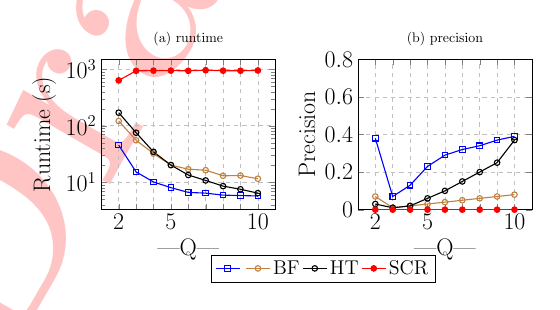
\begin{tikzpicture}[scale=0.5]
  \begin{groupplot}[xtick=data, group style={group size=2 by 1 , horizontal sep=1.0cm}, width = 10cm, every node near coord/.append ,nodes near coords, point meta=explicit symbolic, log origin=infty]%style={yshift=-0.21cm}
    % baseline
    % TR
    % AugX
    
    \nextgroupplot [title = (a) runtime,
    	xlabel={|Q|},
    	ylabel={Runtime (s)},
    	label style={font=\LARGE},
    	tick label style={font=\LARGE},
    % 	legend style={font=\LARGE},
    	legend style={legend columns=2,at={(0.5,-0.2)},anchor=north,font=\Large},
    	width = 6cm,
    	height = 5.4cm,
    	xmin=1,
    	xmax=11,
    	ymin= 0,
    	ymax=1500,
    % 	log basis x={2},
    % 	log basis y={10}, 
    % 	xticklabels={1, , 5,,,,15,,,},
        every axis plot/.append style={thick},
    	ymode=log,
    	xtick={2, 3, 4, 5, 6, 7, 8, 9, 10},
    	ytick={0, 1, 10, 100, 1000},
    	xticklabels={2,,,5,,,,,10,,,,,15},
    	xmajorgrids=true,
    	ymajorgrids=true,
    % 	legend style={at={(1.4,0.7)},anchor=north,font=\LARGE},
    	grid style=dashed]
    	\addplot[color=blue,mark=square] coordinates{(2, 45.4)(3, 15.2)(4, 10.1)(5, 8)(6, 6.6)(7, 6.4)(8, 5.9)(9, 5.8)(10, 5.7)};% \addlegendentry{\hash}
    	\addplot[color=brown,mark=o] coordinates{(2, 121.4)(3, 55.2)(4, 32.2)(5, 20.1)(6, 16.97)(7, 16.3)(8, 13)(9, 13.1)(10, 11.52)}; %\addlegendentry{BF}
    	\addplot[color=black,mark=o] coordinates{(2, 170.1)(3, 75.2)(4, 34.5)(5, 20.1)(6, 13.4)(7, 10.74)(8, 8.52)(9, 7.5)(10, 6.4)}; %\addlegendentry{HT}
        \addplot[color=red,mark=*] coordinates{(2, 634.8)(3, 938.5)(4, 945.9)(5, 946.1)(6, 938.6)(7, 962.3)(8, 943.1)(9, 939.9)(10, 952.1)}; %\addlegendentry{DXF}

    \nextgroupplot [title = (b) precision,
    style={xshift=1.1cm},
    	xlabel={|Q|},
    	ylabel={Precision},
    	label style={font=\LARGE},
    	tick label style={font=\LARGE},
    % 	legend style={font=\LARGE},
    	legend style={legend columns=5,at={(-0.2,-0.3)},anchor=north,font=\Large},
    	width = 6cm,
    	height = 5.4cm,
    	xmin=1,
    	xmax=11,
    	ymin= 0,
    	ymax=.8,
    % 	log basis x={2},
    % 	log basis y={10}, 
    % 	xticklabels={1, , 5,,,,15,,,},
        every axis plot/.append style={thick},
    % 	ymode=log,
    	xtick={2, 3, 4, 5, 6, 7, 8, 9, 10},
    	ytick={0, .2, .4, .6, .8, 1},
    	xticklabels={2,,,5,,,,,10,,,,,15},
    	xmajorgrids=true,
    	ymajorgrids=true,
    % 	legend style={at={(1.4,0.7)},anchor=north,font=\LARGE},
    	grid style=dashed]
    % 	\addplot[color=orange,mark=x] coordinates{(2, 6680)(3, 221)(4, 217)(5, 217)(6, 217)(7, 217)(8, 217)(9, 217)(10, 217)}; \addlegendentry{True positives}
    % 	\addplot[color=blue,mark=square] coordinates{(2, 17587)(3, 3097)(4, 1618)(5, 955)(6, 741)(7, 677)(8, 634)(9, 582)(10, 563)}; \addlegendentry{\hash}
    % 	\addplot[color=brown,mark=o] coordinates{(2, 92883)(3, 23341)(4, 10699)(5, 6440)(6, 5017)(7, 3988)(8, 3483)(9, 3142)(10, 2854)}; \addlegendentry{BF}
    % 	\addplot[color=black,mark=o] coordinates{(2, 211800)(3, 33132)(4, 9645)(5, 3561)(6, 2062)(7, 1405)(8, 1062)(9, 868)(10, 586)}; \addlegendentry{HT}
    %     \addplot[color=red,mark=*] coordinates{(2, 1958951)(3, 1958951)(4, 1958951)(5, 1958951)(6, 1958951)(7, 1958951)(8, 1958951)(9, 1958951)(10, 1958951)}; \addlegendentry{DXF}
        
    	\addplot[color=blue,mark=square] coordinates{(2, .38)(3, .07)(4, .13)(5, .23)(6, .29)(7, .32)(8, .34)(9, .37)(10, .39)}; \addlegendentry{\hash}
    	\addplot[color=brown,mark=o] coordinates{(2, .07)(3, .01)(4, .02)(5, .03)(6, .04)(7, .05)(8, .06)(9, .07)(10, .08)}; \addlegendentry{BF}
    	\addplot[color=black,mark=o] coordinates{(2, .03)(3, .01)(4, .02)(5, .06)(6, .1)(7, .15)(8, .20)(9, .25)(10, .37)}; \addlegendentry{HT}
        \addplot[color=red,mark=*] coordinates{(2, 0)(3, 0)(4, 0)(5, 0)(6, 0)(7, 0)(8, 0)(9, 0)(10, 0)}; \addlegendentry{SCR}
		
  \end{groupplot}
\end{tikzpicture}
% \vspace{-.2cm}
\caption{Key size experiment.}
\label{fig:keysize}
\end{figure}
Here, we evaluate the scalability of \system in the existence of different join-key sizes, i.e.,~the number of columns in the composite key of the input table. 
Due to the limited number of tables with high dimensional composite key, we ran this experiment with a random dataset from the German Open Data corpus with up to 10 columns that can form a composite key (out of 33 columns).
Figure~\ref{fig:keysize} (a) and \ref{fig:keysize} (b) depict the runtime and precision results for different key sizes.
Increasing the number of columns, we observe that the runtime for \system constantly reduces because the FP rate constantly decreases. However, this does not imply a constant increase in precision because increasing the number of key columns changes the ratio of joinable and non-joinable rows. In our experiment, moving from a composite key with two columns to a three-column key, $97\%$ of the joinable rows become non-joinable due to the newly introduced key column. Thus, the filter is confronted with a larger number of FPs, some of which come through.
From key size $4$ upwards, precision increases again as expected.
The runtime gain for larger key sizes is because of two reasons:
\textit{(1)}  With more columns in the query join key, there will be more 1-bits in the query super key, which makes it harder to mask. 
\textit{(2)} Increasing the size of the composite key leads to fewer joinable table rows. Therefore, it is more likely that the second table filtering rule drops the candidate tables without evaluating the remaining rows.
%Again, \hash outperforms other baselines in runtime and precision.   

\subsubsection{Initial column selection.}
%\begin{table}[]
    \small
    \centering
    \caption{Initial query column selection experiment.}
    % \vspace{-.2cm}
    \label{tab:ICS}
\begin{tabular}{l|l|l|l|l|l}
&\textit{\textbf{Best}} & \textit{\textbf{\system}} & \textit{\textbf{Column Order}} & \textit{\textbf{TLS}} & \textit{\textbf{Worst}} \\ \toprule

AVG PL size & 83 & 179 & 202 & 246 & 728

\end{tabular}
\end{table}

We evaluate our heuristic to select the initial query column by comparing the number of retrieved PL items in \system to four other baselines:
\textit{(i)} The column order. In this approach, the initial column will be the first query column according to the column order inside the table. %The idea behind this strategy is that usually, the identifying columns come earlier in the table.
\textit{(ii)} The longest string (TLS). In this approach, the system selects the column that contains the longest cell value as the initial column. %The heuristic here is that the longer the text, the more specific is the column. 
\textit{(iii)} The worst-case scenario. A hypothetical approach that always picks the worst column that returns the larger number of PL items.
\textit{(iv)} Best, i.e. ground truth, which chooses the column that filters most.
The best- and the worst-case scenarios provide lower and upper bounds for our experiment.
This experiment is done using the OD (10k) tables.
In this experiment our cardinality-based heuristic outperfmed the other heuristics. It retrieved on average only 179 PLs compared to Column Order, TLS, and the worst-case scenario with 202, 248, and 728 Pls, respectively. The optimal number of PLs based on ground truth was 83. The heuristic used in \system performs better because of the fact that the number of PL items per cell value follows the power-law distribution. There is a small set of values that have a large number of PL items but most of the values lead to a similar number of PL items (The average number is $12$).
%Table~\ref{tab:ICS} shows that the cardinality-based heuristic used in \system, performs best and is very close to the ground truth approach. The heuristic used in \system performs better because of the fact that the number of PL items per cell value follows the power-law distribution. There is a small set of values that have a large number of PL items but most of the values lead to a similar number of PL items (The average number is $12$).% Thus, there is a direct relationship between the cardinality and the number of retrieved PL items.





\section{Related Work}\label{sec:related}
 
The authors in \cite{humphreys2007noncontact} showed that it is possible to extract the PPG signal from the video using a complementary metal-oxide semiconductor camera by illuminating a region of tissue using through external light-emitting diodes at dual-wavelength (760nm and 880nm).  Further, the authors of  \cite{verkruysse2008remote} demonstrated that the PPG signal can be estimated by just using ambient light as a source of illumination along with a simple digital camera.  Further in \cite{poh2011advancements}, the PPG waveform was estimated from the videos recorded using a low-cost webcam. The red, green, and blue channels of the images were decomposed into independent sources using independent component analysis. One of the independent sources was selected to estimate PPG and further calculate HR, and HRV. All these works showed the possibility of extracting PPG signals from the videos and proved the similarity of this signal with the one obtained using a contact device. Further, the authors in \cite{10.1109/CVPR.2013.440} showed that heart rate can be extracted from features from the head as well by capturing the subtle head movements that happen due to blood flow.

%
The authors of \cite{kumar2015distanceppg} proposed a methodology that overcomes a challenge in extracting PPG for people with darker skin tones. The challenge due to slight movement and low lighting conditions during recording a video was also addressed. They implemented the method where PPG signal is extracted from different regions of the face and signal from each region is combined using their weighted average making weights different for different people depending on their skin color. 
%

There are other attempts where authors of \cite{6523142,6909939, 7410772, 7412627} have introduced different methodologies to make algorithms for estimating pulse rate robust to illumination variation and motion of the subjects. The paper \cite{6523142} introduces a chrominance-based method to reduce the effect of motion in estimating pulse rate. The authors of \cite{6909939} used a technique in which face tracking and normalized least square adaptive filtering is used to counter the effects of variations due to illumination and subject movement. 
The paper \cite{7410772} resolves the issue of subject movement by choosing the rectangular ROI's on the face relative to the facial landmarks and facial landmarks are tracked in the video using pose-free facial landmark fitting tracker discussed in \cite{yu2016face} followed by the removal of noise due to illumination to extract noise-free PPG signal for estimating pulse rate. 

Recently, the use of machine learning in the prediction of health parameters have gained attention. The paper \cite{osman2015supervised} used a supervised learning methodology to predict the pulse rate from the videos taken from any off-the-shelf camera. Their model showed the possibility of using machine learning methods to estimate the pulse rate. However, our method outperforms their results when the root mean squared error of the predicted pulse rate is compared. The authors in \cite{hsu2017deep} proposed a deep learning methodology to predict the pulse rate from the facial videos. The researchers trained a convolutional neural network (CNN) on the images generated using Short-Time Fourier Transform (STFT) applied on the R, G, \& B channels from the facial region of interests.
The authors of \cite{osman2015supervised, hsu2017deep} only predicted pulse rate, and we extended our work in predicting variance in the pulse rate measurements as well.

All the related work discussed above utilizes filtering and digital signal processing to extract PPG signals from the video which is further used to estimate the PR and PRV.  %
The method proposed in \cite{kumar2015distanceppg} is person dependent since the weights will be different for people with different skin tone. In contrast, we propose a deep learning model to predict the PR which is independent of the person who is being trained. Thus, the model would work even if there is no prior training model built for that individual and hence, making our model robust. 

%
\section{Conclusion and Future Work} \label{sec:conclusion}
In this paper, we tackled the problem of n-ary or multi-attribute join search. We proposed a hash-based filtering approach \system that removes redundant table rows from further joinability calculation processes to increase the scalability of the join discovery. We proposed \hash, a hash function that leverages syntactic features of the cell values that ultimately lead to the lowest FP rates. We showed that \system is more effective and efficient than state-of-the-art systems.
We focused on the equi-joins. Because \hash uses syntactic features including the character and length features of the cell values, it has the potential to discover similarity joins as well. According to our observations, the false positives caused by \hash were those that are syntactically similar to the actual key values, e.g., discovering the composite key <``brooklyn'', ``cambridge''> instead of <``brooklyn'', ``bay ridge''>. 
Another future direction is to reason about hashing short key values. \hash cannot use its optimal potential if cell values are too short.


\begin{acks} 
This project has been supported by the German Research Foundation (DFG) under grant agreement 387872445 and the German Ministry for Education and Research as BIFOLD — “Berlin Institute for the Foundations of Learning and Data” (01IS18025A and 01IS18037A).
\end{acks}

\balance

% \small
%\bibliographystyle{abbrv}
 \bibliographystyle{ACM-Reference-Format}
\bibliography{references}

\end{document}
